% Options for packages loaded elsewhere
\PassOptionsToPackage{unicode}{hyperref}
\PassOptionsToPackage{hyphens}{url}
% Compile with XeLaTeX on Overleaf
\documentclass[
]{article}
\usepackage{xcolor}
\usepackage{amsmath,amssymb}
\setcounter{secnumdepth}{-\maxdimen} % remove section numbering
\usepackage{fontspec}
\usepackage{polyglossia}
\setmainlanguage{vietnamese}
\setotherlanguage{english}
\setmainfont{Times New Roman}

% Use upquote if available, for straight quotes in verbatim environments
\IfFileExists{upquote.sty}{\usepackage{upquote}}{}
\IfFileExists{microtype.sty}{% use microtype if available
  \usepackage[]{microtype}
  \UseMicrotypeSet[protrusion]{basicmath} % disable protrusion for tt fonts
}{}
\makeatletter
\@ifundefined{KOMAClassName}{% if non-KOMA class
  \IfFileExists{parskip.sty}{%
    \usepackage{parskip}
  }{% else
    \setlength{\parindent}{0pt}
    \setlength{\parskip}{6pt plus 2pt minus 1pt}}
}{% if KOMA class
  \KOMAoptions{parskip=half}}
\makeatother
\usepackage{color}
\usepackage{fancyvrb}
\newcommand{\VerbBar}{|}
\newcommand{\VERB}{\Verb[commandchars=\\\{\}]}
\DefineVerbatimEnvironment{Highlighting}{Verbatim}{commandchars=\\\{\}}
% Add ',fontsize=\small' for more characters per line
\newenvironment{Shaded}{}{}
\newcommand{\AlertTok}[1]{\textcolor[rgb]{1.00,0.00,0.00}{\textbf{#1}}}
\newcommand{\AnnotationTok}[1]{\textcolor[rgb]{0.38,0.63,0.69}{\textbf{\textit{#1}}}}
\newcommand{\AttributeTok}[1]{\textcolor[rgb]{0.49,0.56,0.16}{#1}}
\newcommand{\BaseNTok}[1]{\textcolor[rgb]{0.25,0.63,0.44}{#1}}
\newcommand{\BuiltInTok}[1]{\textcolor[rgb]{0.00,0.50,0.00}{#1}}
\newcommand{\CharTok}[1]{\textcolor[rgb]{0.25,0.44,0.63}{#1}}
\newcommand{\CommentTok}[1]{\textcolor[rgb]{0.38,0.63,0.69}{\textit{#1}}}
\newcommand{\CommentVarTok}[1]{\textcolor[rgb]{0.38,0.63,0.69}{\textbf{\textit{#1}}}}
\newcommand{\ConstantTok}[1]{\textcolor[rgb]{0.53,0.00,0.00}{#1}}
\newcommand{\ControlFlowTok}[1]{\textcolor[rgb]{0.00,0.44,0.13}{\textbf{#1}}}
\newcommand{\DataTypeTok}[1]{\textcolor[rgb]{0.56,0.13,0.00}{#1}}
\newcommand{\DecValTok}[1]{\textcolor[rgb]{0.25,0.63,0.44}{#1}}
\newcommand{\DocumentationTok}[1]{\textcolor[rgb]{0.73,0.13,0.13}{\textit{#1}}}
\newcommand{\ErrorTok}[1]{\textcolor[rgb]{1.00,0.00,0.00}{\textbf{#1}}}
\newcommand{\ExtensionTok}[1]{#1}
\newcommand{\FloatTok}[1]{\textcolor[rgb]{0.25,0.63,0.44}{#1}}
\newcommand{\FunctionTok}[1]{\textcolor[rgb]{0.02,0.16,0.49}{#1}}
\newcommand{\ImportTok}[1]{\textcolor[rgb]{0.00,0.50,0.00}{\textbf{#1}}}
\newcommand{\InformationTok}[1]{\textcolor[rgb]{0.38,0.63,0.69}{\textbf{\textit{#1}}}}
\newcommand{\KeywordTok}[1]{\textcolor[rgb]{0.00,0.44,0.13}{\textbf{#1}}}
\newcommand{\NormalTok}[1]{#1}
\newcommand{\OperatorTok}[1]{\textcolor[rgb]{0.40,0.40,0.40}{#1}}
\newcommand{\OtherTok}[1]{\textcolor[rgb]{0.00,0.44,0.13}{#1}}
\newcommand{\PreprocessorTok}[1]{\textcolor[rgb]{0.74,0.48,0.00}{#1}}
\newcommand{\RegionMarkerTok}[1]{#1}
\newcommand{\SpecialCharTok}[1]{\textcolor[rgb]{0.25,0.44,0.63}{#1}}
\newcommand{\SpecialStringTok}[1]{\textcolor[rgb]{0.73,0.40,0.53}{#1}}
\newcommand{\StringTok}[1]{\textcolor[rgb]{0.25,0.44,0.63}{#1}}
\newcommand{\VariableTok}[1]{\textcolor[rgb]{0.10,0.09,0.49}{#1}}
\newcommand{\VerbatimStringTok}[1]{\textcolor[rgb]{0.25,0.44,0.63}{#1}}
\newcommand{\WarningTok}[1]{\textcolor[rgb]{0.38,0.63,0.69}{\textbf{\textit{#1}}}}
\usepackage{longtable,booktabs,array}
\newcounter{none} % for unnumbered tables
\usepackage{calc} % for calculating minipage widths
% Correct order of tables after \paragraph or \subparagraph
\usepackage{etoolbox}
\makeatletter
\patchcmd\longtable{\par}{\if@noskipsec\mbox{}\fi\par}{}{}
\makeatother
% Allow footnotes in longtable head/foot
\IfFileExists{footnotehyper.sty}{\usepackage{footnotehyper}}{\usepackage{footnote}}
\makesavenoteenv{longtable}
\usepackage{graphicx}
\graphicspath{{assets/}}
\makeatletter
\newsavebox\pandoc@box
\newcommand*\pandocbounded[1]{% scales image to fit in text height/width
  \sbox\pandoc@box{#1}%
  \Gscale@div\@tempa{\textheight}{\dimexpr\ht\pandoc@box+\dp\pandoc@box\relax}%
  \Gscale@div\@tempb{\linewidth}{\wd\pandoc@box}%
  \ifdim\@tempb\p@<\@tempa\p@\let\@tempa\@tempb\fi% select the smaller of both
  \ifdim\@tempa\p@<\p@\scalebox{\@tempa}{\usebox\pandoc@box}%
  \else\usebox{\pandoc@box}%
  \fi%
}
% Set default figure placement to htbp
\def\fps@figure{htbp}
\makeatother
\setlength{\emergencystretch}{3em} % prevent overfull lines
\providecommand{\tightlist}{%
  \setlength{\itemsep}{0pt}\setlength{\parskip}{0pt}}
\usepackage{bookmark}
\IfFileExists{xurl.sty}{\usepackage{xurl}}{} % add URL line breaks if available
\urlstyle{same}
\hypersetup{
  hidelinks,
  pdfcreator={LaTeX via pandoc}}

\author{}
\date{}

\begin{document}

\section{Báo Cáo Bài Tập Lớn Môn Học
Máy}\label{buxe1o-cuxe1o-buxe0i-tux1eadp-lux1edbn-muxf4n-hux1ecdc-muxe1y}

\subsection{Adult Census Income Prediction
Pipeline}\label{adult-census-income-prediction-pipeline}

\begin{center}\rule{0.5\linewidth}{0.5pt}\end{center}

\subsection{Thông Tin Chung}\label{thuxf4ng-tin-chung}

{\def\LTcaptype{none} % do not increment counter
\begin{longtable}[]{@{}ll@{}}
\toprule\noalign{}
Mục & Chi tiết \\
\midrule\noalign{}
\endhead
\bottomrule\noalign{}
\endlastfoot
\textbf{Môn học} & Nhập môn Học Máy \\
\textbf{Mã môn học} & \emph{(Vui lòng cập nhật mã môn)} \\
\textbf{Trường} & Đại học Bách Khoa TP.HCM (HCMUT) \\
\textbf{Học kỳ} & HK2 - Năm học 2025-2026 \\
\textbf{GVHD} & TS. Lê Thành Sách \\
\textbf{Nhóm} & \emph{(Vui lòng điền tên nhóm + thành viên + MSSV)} \\
\end{longtable}
}

\begin{center}\rule{0.5\linewidth}{0.5pt}\end{center}

\subsection{1. Tóm Tắt (Abstract)}\label{1-tuxf3m-tux1eaft-abstract}

Bài tập lớn này xây dựng một \textbf{Machine Learning Pipeline} hoàn
chỉnh để giải quyết bài toán phân loại nhị phân: \textbf{dự đoán thu
nhập cá nhân có vượt 50K\$ hay không} (Adult Census Income dataset).
Pipeline bao gồm các bước chính:

\begin{enumerate}
\def\labelenumi{\arabic{enumi}.}
\tightlist
\item
  \textbf{Khám phá dữ liệu (EDA):} Trực quan hóa phân phối biến số
  (Boxplot), ma trận tương quan (Correlation Heatmap), và phân tích biến
  phân loại (CountPlot) để hiểu đặc điểm dữ liệu.
\item
  \textbf{Tiền xử lý dữ liệu:} Xử lý giá trị khuyết (missing values)
  bằng \texttt{SimpleImputer}, mã hóa biến phân loại bằng
  \texttt{OneHotEncoder}, và chuẩn hóa biến số bằng
  \texttt{StandardScaler}.
\item
  \textbf{Xử lý mất cân bằng dữ liệu:} Áp dụng kỹ thuật \textbf{SMOTE}
  (Synthetic Minority Over-sampling Technique) để tăng cường lớp thiểu
  số.
\item
  \textbf{So sánh mô hình truyền thống:} Huấn luyện và đánh giá 4 mô
  hình: \texttt{Logistic\ Regression}, \texttt{Random\ Forest},
  \texttt{Linear\ SVM}, và \texttt{LightGBM} với các chỉ số Accuracy,
  ROC-AUC, và thời gian huấn luyện.
\item
  \textbf{Mở rộng Deep Learning:} Xây dựng mạng nơ-ron MLP (Multi-Layer
  Perceptron) bằng PyTorch với class weights để xử lý imbalanced data.
\item
  \textbf{Trực quan hóa và đánh giá:} So sánh hiệu suất giữa mô hình
  truyền thống và deep learning thông qua Bar Chart, ROC Curve, và
  Confusion Matrix.
\item
  \textbf{Export đặc trưng:} Lưu các vector đặc trưng đã xử lý và mô
  hình đã huấn luyện dưới dạng \texttt{.npy}, \texttt{.pkl}, và
  \texttt{.pth} để tái sử dụng.
\end{enumerate}

\textbf{Kết quả nổi bật:} Mô hình \textbf{LightGBM} đạt hiệu suất tốt
nhất trong các mô hình truyền thống với \textbf{Accuracy = 0.842} và
\textbf{ROC-AUC = 0.921}. Mô hình MLP Deep Learning đạt \textbf{Accuracy
= 0.806} và \textbf{ROC-AUC = 0.906}, cho thấy cả hai hướng tiếp cận đều
hiệu quả nhưng LightGBM vượt trội hơn về độ chính xác và thời gian huấn
luyện.

\begin{center}\rule{0.5\linewidth}{0.5pt}\end{center}

\subsection{2. Mục Tiêu Bài Làm}\label{2-mux1ee5c-tiuxeau-buxe0i-luxe0m}

Theo yêu cầu từ tài liệu \texttt{mlAssignments\_v1.1.pdf}, bài tập lớn
cần đáp ứng các tiêu chí sau:

\subsubsection{2.1. Yêu Cầu Bắt Buộc (Pipeline Truyền
Thống)}\label{21-yuxeau-cux1ea7u-bux1eaft-buux1ed9c-pipeline-truyux1ec1n-thux1ed1ng}

\begin{itemize}
\item
  \textbf{EDA (Exploratory Data Analysis):} Thực hiện phân tích khám phá
  dữ liệu bắt buộc, bao gồm:

  \begin{itemize}
  \tightlist
  \item
    Boxplot để phát hiện outliers trong biến số
  \item
    Correlation Heatmap để xem xét mối tương quan giữa các biến
  \item
    CountPlot để phân tích phân phối biến phân loại
  \end{itemize}
\item
  \textbf{Tiền xử lý dữ liệu:}

  \begin{itemize}
  \tightlist
  \item
    Xử lý missing values (dữ liệu có chứa ký tự \texttt{?} cần được xử
    lý bằng imputation)
  \item
    Encoding cho biến categorical (OneHotEncoder)
  \item
    Scaling cho biến numeric (StandardScaler hoặc MinMaxScaler)
  \end{itemize}
\item
  \textbf{Xử lý Imbalanced Data:}

  \begin{itemize}
  \tightlist
  \item
    Áp dụng kỹ thuật SMOTE để cân bằng tỉ lệ lớp
  \end{itemize}
\item
  \textbf{So sánh mô hình:}

  \begin{itemize}
  \tightlist
  \item
    Huấn luyện và so sánh ít nhất 4 mô hình truyền thống (Logistic
    Regression, Random Forest, Linear SVM, LightGBM)
  \item
    Đánh giá bằng các chỉ số: Accuracy, ROC-AUC, F1-Score
  \end{itemize}
\item
  \textbf{Trực quan hóa:}

  \begin{itemize}
  \tightlist
  \item
    Bar Chart so sánh các chỉ số giữa các mô hình
  \item
    ROC Curve
  \item
    Confusion Matrix
  \end{itemize}
\item
  \textbf{Export đặc trưng:}

  \begin{itemize}
  \tightlist
  \item
    Lưu các vector đặc trưng đã xử lý dưới dạng \texttt{.npy}
  \item
    Lưu mô hình đã huấn luyện dưới dạng \texttt{.pkl}
  \end{itemize}
\end{itemize}

\subsubsection{2.2. Yêu Cầu Mở Rộng (Điểm
Cộng)}\label{22-yuxeau-cux1ea7u-mux1edf-rux1ed9ng-ux111iux1ec3m-cux1ed9ng}

\begin{itemize}
\tightlist
\item
  \textbf{Pipeline Deep Learning:} Xây dựng mô hình MLP bằng PyTorch và
  so sánh với pipeline truyền thống (+5\% điểm)
\item
  \textbf{Công bố trên GitHub:} Tổ chức dự án đầy đủ với README, hướng
  dẫn chạy, và link Colab (+5\% điểm)
\end{itemize}

Bài làm của nhóm đã \textbf{đáp ứng đầy đủ} các yêu cầu bắt buộc và
\textbf{hoàn thành cả 2 yêu cầu mở rộng} để tối đa hóa điểm số.

\begin{center}\rule{0.5\linewidth}{0.5pt}\end{center}

\subsection{3. Dữ Liệu và Khám Phá Dữ Liệu
(EDA)}\label{3-dux1eef-liux1ec7u-vuxe0-khuxe1m-phuxe1-dux1eef-liux1ec7u-eda}

\subsubsection{3.1. Mô Tả Dataset}\label{31-muxf4-tux1ea3-dataset}

\begin{itemize}
\tightlist
\item
  \textbf{Tên dataset:} Adult Census Income
\item
  \textbf{Nguồn:} Kaggle -
  \href{https://www.kaggle.com/datasets/uciml/adult-census-income}{uciml/adult-census-income}
\item
  \textbf{Kích thước:} 32,561 mẫu với 15 thuộc tính (14 features + 1
  target)
\item
  \textbf{Phương thức tải:} Tự động thông qua thư viện
  \texttt{kagglehub} (không cần mount Google Drive)
\end{itemize}

\textbf{Các thuộc tính chính:}

\textbf{Biến số (Numeric):}

\begin{itemize}
\tightlist
\item
  \texttt{age}: Tuổi
\item
  \texttt{fnlwgt}: Final weight (trọng số mẫu)
\item
  \texttt{education.num}: Số năm học
\item
  \texttt{capital.gain}: Lợi nhuận vốn
\item
  \texttt{capital.loss}: Lỗ vốn
\item
  \texttt{hours.per.week}: Số giờ làm việc mỗi tuần
\end{itemize}

\textbf{Biến phân loại (Categorical):}

\begin{itemize}
\tightlist
\item
  \texttt{workclass}: Loại công việc (Private, Self-emp, Government,
  ...)
\item
  \texttt{education}: Trình độ học vấn (HS-grad, Bachelors, Masters,
  ...)
\item
  \texttt{marital.status}: Tình trạng hôn nhân
\item
  \texttt{occupation}: Nghề nghiệp
\item
  \texttt{relationship}: Mối quan hệ trong gia đình
\item
  \texttt{race}: Chủng tộc
\item
  \texttt{sex}: Giới tính
\item
  \texttt{native.country}: Quốc gia xuất xứ
\end{itemize}

\textbf{Target:}

\begin{itemize}
\tightlist
\item
  \texttt{income}: Thu nhập (\texttt{\textless{}=50K} hoặc
  \texttt{\textgreater{}50K}), được chuyển đổi thành nhãn nhị phân (0/1)
\end{itemize}

\subsubsection{3.2. Tiền Xử Lý Cho
EDA}\label{32-tiux1ec1n-xux1eed-luxfd-cho-eda}

Trước khi thực hiện EDA, dữ liệu được làm sạch sơ bộ:

\begin{enumerate}
\def\labelenumi{\arabic{enumi}.}
\tightlist
\item
  \textbf{Xử lý ký tự \texttt{?}:} Các giá trị \texttt{?} trong dữ liệu
  được thay thế bằng \texttt{np.nan} để đánh dấu missing values.
\item
  \textbf{Chuẩn hóa target:} Nhãn \texttt{income} được chuyển từ chuỗi
  \texttt{\textquotesingle{}\textgreater{}50K\textquotesingle{}} và
  \texttt{\textquotesingle{}\textless{}=50K\textquotesingle{}} thành giá
  trị nhị phân \texttt{1} và \texttt{0}.
\end{enumerate}

\textbf{Thống kê missing values:}

\begin{verbatim}
Missing Values:
workclass         1836
occupation        1843
native.country     583
\end{verbatim}

Các cột \texttt{workclass}, \texttt{occupation}, và
\texttt{native.country} có missing values đáng kể, cần được xử lý bằng
imputation trong bước tiền xử lý.

\subsubsection{3.3. EDA Bắt Buộc}\label{33-eda-bux1eaft-buux1ed9c}

\paragraph{3.3.1. Boxplot - Phát Hiện
Outliers}\label{331-boxplot---phuxe1t-hiux1ec7n-outliers}

\pandocbounded{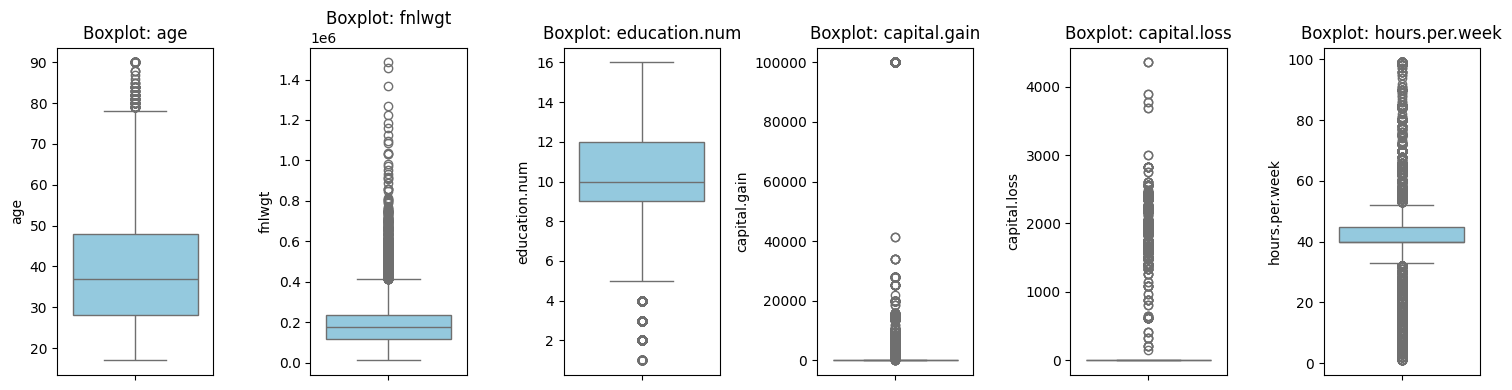
\includegraphics[keepaspectratio,alt={Boxplot}]{assets/fig_01_cell7_out0.png}}

\textbf{Phân tích:}

\begin{itemize}
\tightlist
\item
  \textbf{\texttt{age}:} Phân phối tương đối đồng đều, không có outliers
  nghiêm trọng.
\item
  \textbf{\texttt{fnlwgt}:} Có một số outliers ở giá trị cao, nhưng đây
  là trọng số mẫu nên không cần xử lý.
\item
  \textbf{\texttt{education.num}:} Phân phối tập trung ở các giá trị từ
  9-13 (tương ứng HS-grad đến Bachelors).
\item
  \textbf{\texttt{capital.gain} và \texttt{capital.loss}:} Hầu hết giá
  trị đều bằng 0, chỉ một số ít mẫu có giá trị khác 0 (outliers rõ
  ràng). Đây là đặc điểm tự nhiên của dữ liệu tài chính, không cần loại
  bỏ.
\item
  \textbf{\texttt{hours.per.week}:} Phân phối tập trung quanh 40
  giờ/tuần (full-time), có một số outliers ở giá trị thấp và cao.
\end{itemize}

\textbf{Kết luận:} Không có outliers nghiêm trọng cần loại bỏ. Các
outliers trong \texttt{capital.gain} và \texttt{capital.loss} là đặc
điểm tự nhiên của dữ liệu và có thể chứa thông tin quan trọng cho mô
hình.

\paragraph{3.3.2. Correlation Heatmap - Ma Trận Tương
Quan}\label{332-correlation-heatmap---ma-trux1eadn-tux1b0ux1a1ng-quan}

\pandocbounded{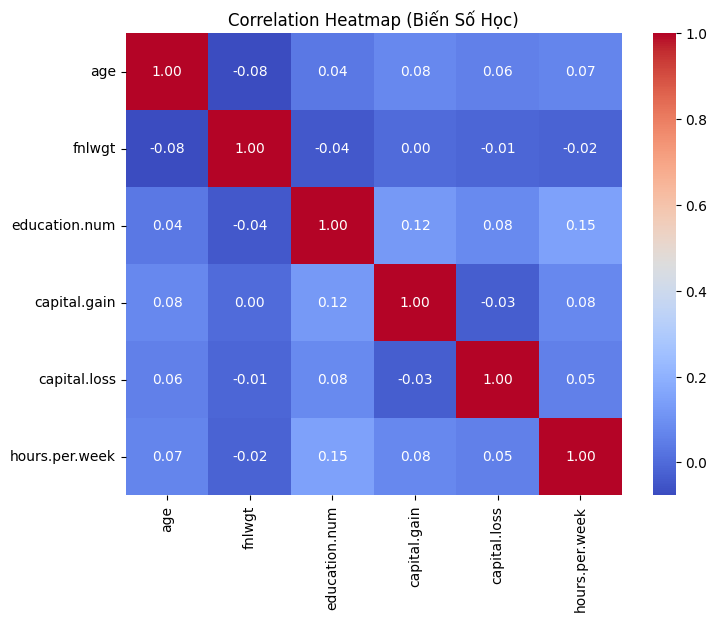
\includegraphics[keepaspectratio,alt={Correlation Heatmap}]{assets/fig_02_cell7_out1.png}}

\textbf{Phân tích:}

\begin{itemize}
\tightlist
\item
  \textbf{Tương quan mạnh nhất:} \texttt{education.num} và \texttt{age}
  có tương quan dương yếu (\textasciitilde0.04), cho thấy người lớn tuổi
  hơn có xu hướng có trình độ học vấn cao hơn (nhưng không mạnh).
\item
  \textbf{\texttt{capital.gain} và \texttt{capital.loss}:} Có tương quan
  rất yếu với các biến khác, cho thấy đây là các biến độc lập và có thể
  mang thông tin riêng biệt.
\item
  \textbf{Không có multicollinearity nghiêm trọng:} Không có cặp biến
  nào có tương quan tuyến tính quá cao (\textgreater0.8), do đó không
  cần loại bỏ biến để giảm multicollinearity.
\end{itemize}

\textbf{Kết luận:} Các biến số có tương quan tuyến tính yếu với nhau,
cho thấy mỗi biến đều mang thông tin riêng biệt và có thể đóng góp vào
mô hình.

\paragraph{3.3.3. CountPlot - Phân Tích Biến Phân
Loại}\label{333-countplot---phuxe2n-tuxedch-biux1ebfn-phuxe2n-loux1ea1i}

\pandocbounded{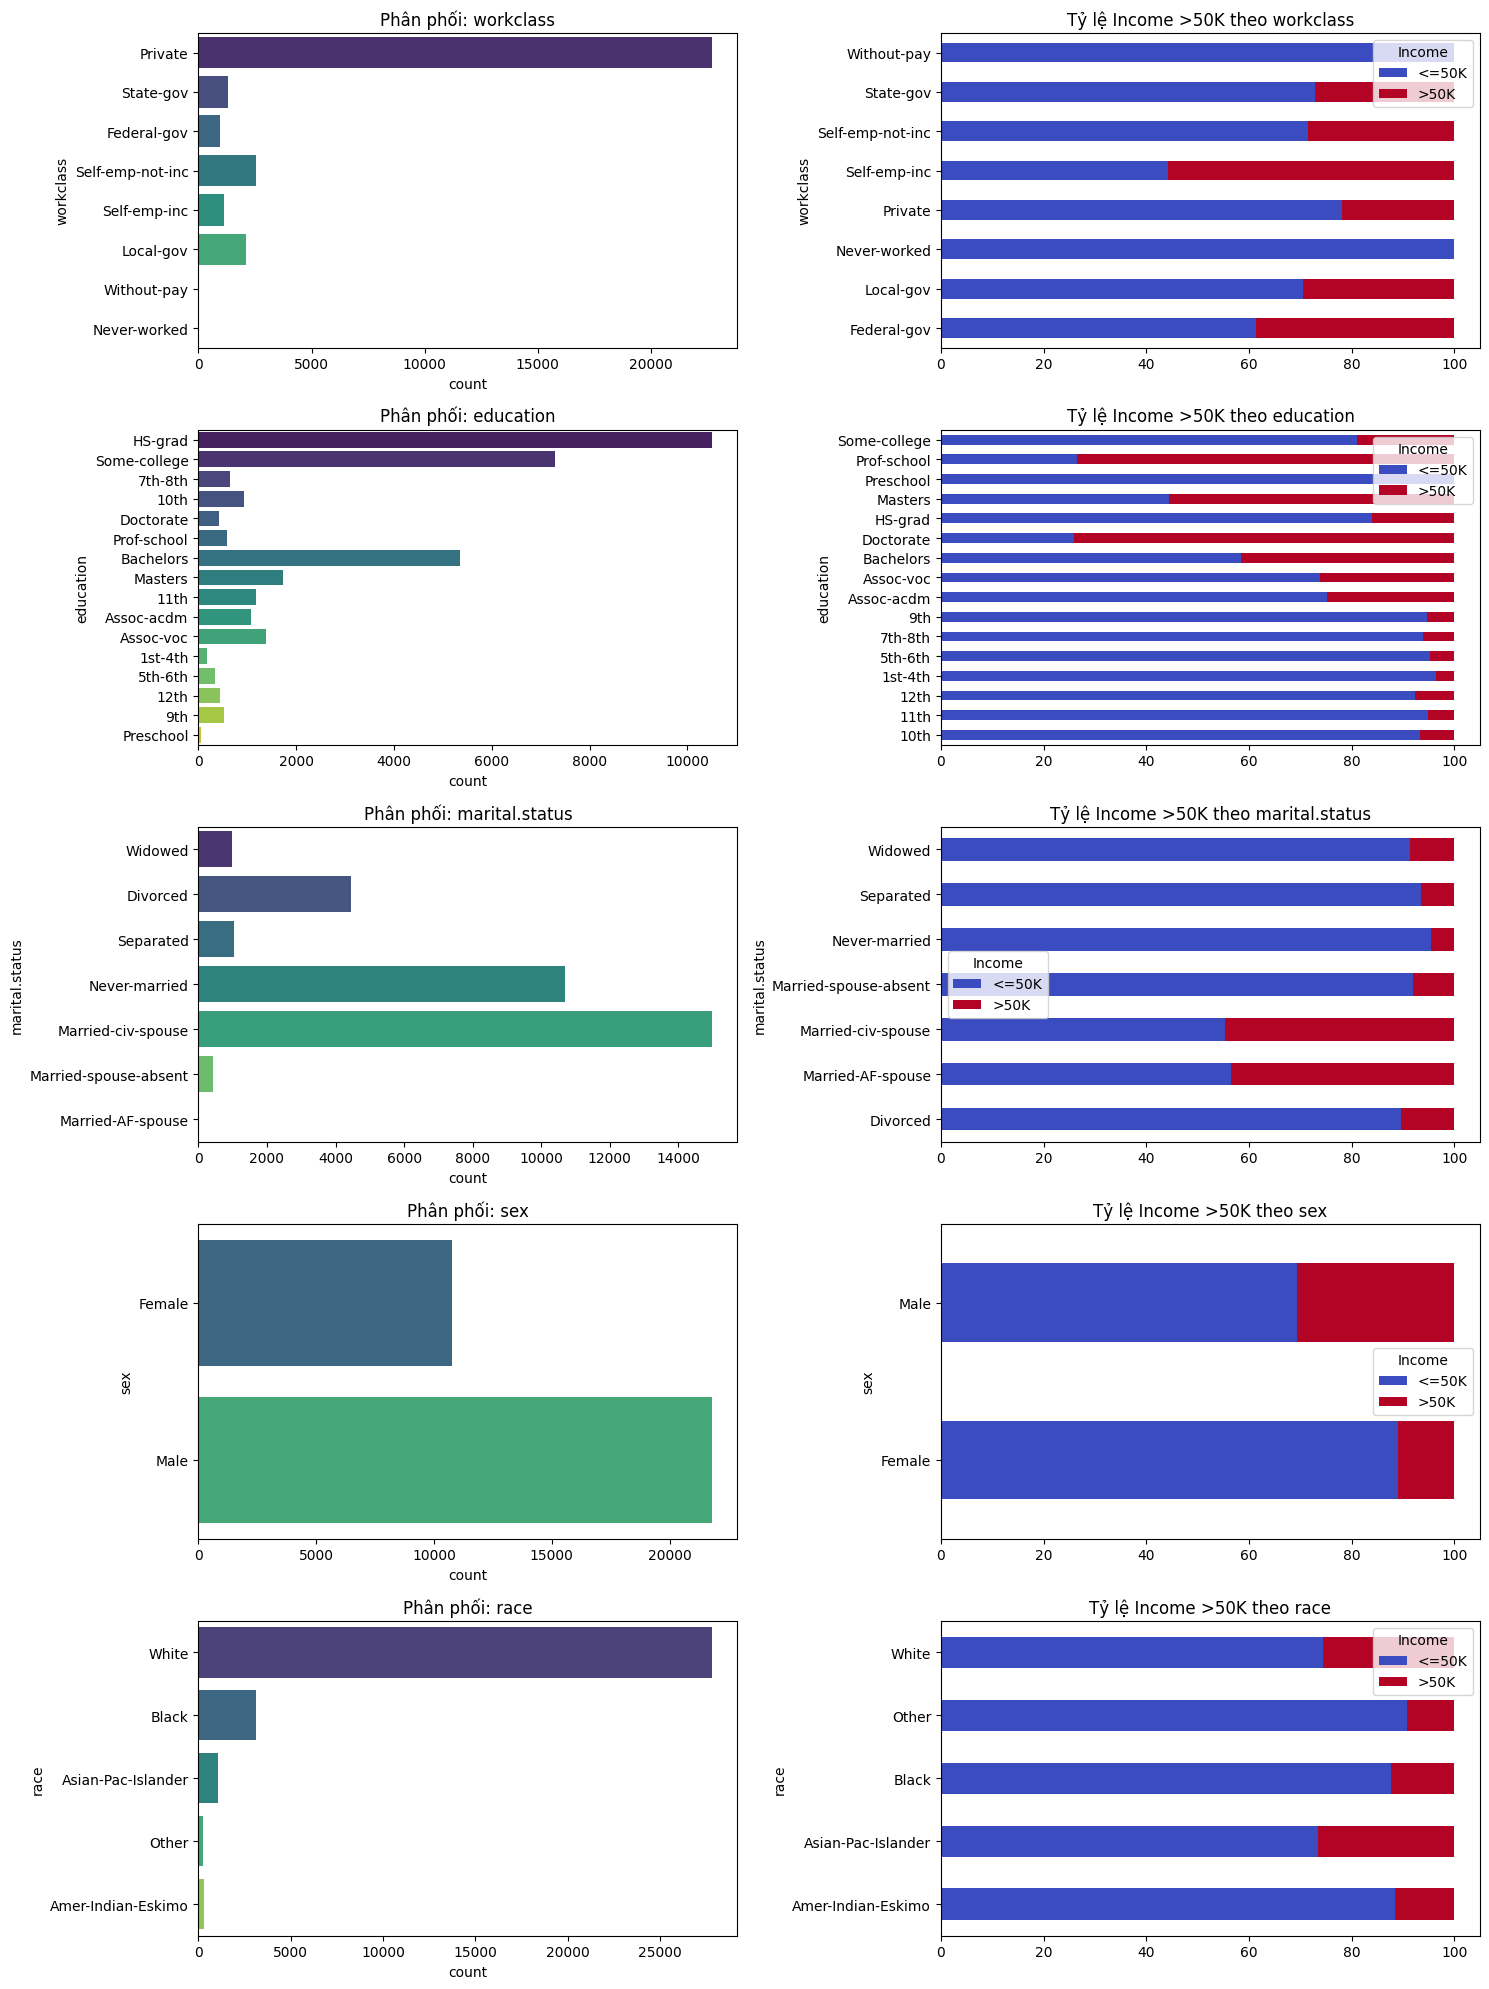
\includegraphics[keepaspectratio,alt={CountPlot}]{assets/fig_03_cell9_out0.png}}

\textbf{Phân tích:}

\textbf{\texttt{workclass}:}

\begin{itemize}
\tightlist
\item
  Phần lớn mẫu thuộc nhóm \texttt{Private} (khoảng 70\%), tiếp theo là
  \texttt{Self-emp-not-inc} và \texttt{Local-gov}.
\item
  Tỉ lệ thu nhập \textgreater50K cao nhất ở nhóm \texttt{Self-emp-inc}
  (tự kinh doanh có đăng ký).
\end{itemize}

\textbf{\texttt{education}:}

\begin{itemize}
\tightlist
\item
  Phân phối tập trung ở \texttt{HS-grad} (tốt nghiệp trung học) và
  \texttt{Some-college}.
\item
  Tỉ lệ thu nhập \textgreater50K tăng mạnh theo trình độ học vấn:
  \texttt{Bachelors}, \texttt{Masters}, \texttt{Doctorate} có tỉ lệ
  \textgreater50K cao nhất.
\end{itemize}

\textbf{\texttt{marital.status}:}

\begin{itemize}
\tightlist
\item
  Nhóm \texttt{Married-civ-spouse} (đã kết hôn) chiếm đa số và có tỉ lệ
  thu nhập \textgreater50K cao nhất (\textasciitilde45\%).
\item
  Các nhóm \texttt{Never-married}, \texttt{Divorced}, \texttt{Separated}
  có tỉ lệ thu nhập \textgreater50K thấp hơn nhiều (\textless15\%).
\end{itemize}

\textbf{\texttt{sex}:}

\begin{itemize}
\tightlist
\item
  Số lượng nam (\texttt{Male}) nhiều hơn nữ (\texttt{Female}) gần gấp
  đôi.
\item
  Tỉ lệ thu nhập \textgreater50K ở nam (\textasciitilde30\%) cao hơn nữ
  (\textasciitilde10\%) đáng kể, phản ánh sự bất bình đẳng giới trong
  thu nhập.
\end{itemize}

\textbf{\texttt{race}:}

\begin{itemize}
\tightlist
\item
  Phần lớn mẫu thuộc nhóm \texttt{White} (\textasciitilde85\%), tiếp
  theo là \texttt{Black} và \texttt{Asian-Pac-Islander}.
\item
  Tỉ lệ thu nhập \textgreater50K ở các nhóm chủng tộc khá tương đồng,
  nhưng \texttt{Asian-Pac-Islander} có tỉ lệ cao hơn một chút.
\end{itemize}

\textbf{Kết luận:} Các biến phân loại có ảnh hưởng rõ ràng đến thu nhập,
đặc biệt là \texttt{education}, \texttt{marital.status}, và
\texttt{sex}. Điều này cho thấy các biến này sẽ là đặc trưng quan trọng
cho mô hình phân loại.

\subsubsection{3.4. Phân Tích Mất Cân Bằng (Imbalanced
Data)}\label{34-phuxe2n-tuxedch-mux1ea5t-cuxe2n-bux1eb1ng-imbalanced-data}

\textbf{Phân phối target trước SMOTE:}

\begin{itemize}
\tightlist
\item
  \texttt{income\ \textless{}=\ 50K} (lớp 0): 24,720 mẫu
  (\textasciitilde76\%)
\item
  \texttt{income\ \textgreater{}\ 50K} (lớp 1): 7,841 mẫu
  (\textasciitilde24\%)
\end{itemize}

\textbf{Tỉ lệ:} Lớp thiểu số (\textgreater50K) chỉ chiếm khoảng 1/3 lớp
đa số, cho thấy dữ liệu \textbf{mất cân bằng vừa phải}. Nếu không xử lý,
mô hình có thể bị bias về lớp đa số (\textless=50K) và dự đoán kém cho
lớp thiểu số (\textgreater50K).

\textbf{Giải pháp:} Áp dụng \textbf{SMOTE} với
\texttt{sampling\_strategy=0.5} để tăng số lượng mẫu lớp thiểu số lên
50\% số lượng lớp đa số, giúp cân bằng dữ liệu mà không gây overfitting
như random oversampling.

\begin{center}\rule{0.5\linewidth}{0.5pt}\end{center}

\subsection{4. Phương Pháp (Pipeline) và Thiết Kế Thí
Nghiệm}\label{4-phux1b0ux1a1ng-phuxe1p-pipeline-vuxe0-thiux1ebft-kux1ebf-thuxed-nghiux1ec7m}

\subsubsection{4.1. Pipeline Truyền Thống (Traditional ML
Pipeline)}\label{41-pipeline-truyux1ec1n-thux1ed1ng-traditional-ml-pipeline}

\paragraph{4.1.1. Split Train/Test}\label{411-split-traintest}

Dữ liệu được chia thành tập train và test với tỉ lệ 80/20:

\begin{Shaded}
\begin{Highlighting}[]
\NormalTok{X\_train, X\_test, y\_train, y\_test }\OperatorTok{=}\NormalTok{ train\_test\_split(}
\NormalTok{    X, y, test\_size}\OperatorTok{=}\FloatTok{0.2}\NormalTok{, random\_state}\OperatorTok{=}\DecValTok{42}\NormalTok{, stratify}\OperatorTok{=}\NormalTok{y}
\NormalTok{)}
\end{Highlighting}
\end{Shaded}

\textbf{Lý do sử dụng \texttt{stratify=y}:} Đảm bảo tỉ lệ lớp trong tập
train và test giống nhau với tập gốc, tránh tình trạng tập test có phân
phối khác biệt so với tập train.

\textbf{Kết quả:}

\begin{itemize}
\tightlist
\item
  Tập train: 26,048 mẫu
\item
  Tập test: 6,513 mẫu
\end{itemize}

\paragraph{4.1.2. Preprocessing (Tiền Xử
Lý)}\label{412-preprocessing-tiux1ec1n-xux1eed-luxfd}

Pipeline tiền xử lý được thiết kế theo 3 bước chính:

\textbf{1. Xử lý biến số (Numeric Features):}

\begin{Shaded}
\begin{Highlighting}[]
\NormalTok{num\_transformer }\OperatorTok{=}\NormalTok{ ImbPipeline(steps}\OperatorTok{=}\NormalTok{[}
\NormalTok{    (}\StringTok{\textquotesingle{}imputer\textquotesingle{}}\NormalTok{, SimpleImputer(strategy}\OperatorTok{=}\StringTok{\textquotesingle{}median\textquotesingle{}}\NormalTok{)),}
\NormalTok{    (}\StringTok{\textquotesingle{}scaler\textquotesingle{}}\NormalTok{, StandardScaler())}
\NormalTok{])}
\end{Highlighting}
\end{Shaded}

\begin{itemize}
\tightlist
\item
  \textbf{Imputation:} Thay thế missing values bằng giá trị trung vị
  (median) của cột.
\item
  \textbf{Scaling:} Chuẩn hóa về phân phối chuẩn (mean=0, std=1) để các
  biến có cùng thang đo.
\end{itemize}

\textbf{2. Xử lý biến phân loại (Categorical Features):}

\begin{Shaded}
\begin{Highlighting}[]
\NormalTok{cat\_transformer }\OperatorTok{=}\NormalTok{ ImbPipeline(steps}\OperatorTok{=}\NormalTok{[}
\NormalTok{    (}\StringTok{\textquotesingle{}imputer\textquotesingle{}}\NormalTok{, SimpleImputer(strategy}\OperatorTok{=}\StringTok{\textquotesingle{}constant\textquotesingle{}}\NormalTok{, fill\_value}\OperatorTok{=}\StringTok{\textquotesingle{}Missing\_Value\textquotesingle{}}\NormalTok{)),}
\NormalTok{    (}\StringTok{\textquotesingle{}encoder\textquotesingle{}}\NormalTok{, OneHotEncoder(handle\_unknown}\OperatorTok{=}\StringTok{\textquotesingle{}ignore\textquotesingle{}}\NormalTok{, sparse}\OperatorTok{=}\VariableTok{False}\NormalTok{))}
\NormalTok{])}
\end{Highlighting}
\end{Shaded}

\begin{itemize}
\tightlist
\item
  \textbf{Imputation:} Thay thế missing values bằng một giá trị cố định
  \texttt{\textquotesingle{}Missing\_Value\textquotesingle{}} để đánh
  dấu riêng.
\item
  \textbf{Encoding:} Chuyển đổi biến phân loại thành vector one-hot (mỗi
  category thành một cột binary).
\item
  \textbf{\texttt{handle\_unknown=\textquotesingle{}ignore\textquotesingle{}}:}
  Xử lý các category chưa gặp trong tập train bằng cách gán vector 0.
\end{itemize}

\textbf{3. Ghép nối (ColumnTransformer):}

\begin{Shaded}
\begin{Highlighting}[]
\NormalTok{preprocessor }\OperatorTok{=}\NormalTok{ ColumnTransformer(transformers}\OperatorTok{=}\NormalTok{[}
\NormalTok{    (}\StringTok{\textquotesingle{}num\textquotesingle{}}\NormalTok{, num\_transformer, num\_cols),}
\NormalTok{    (}\StringTok{\textquotesingle{}cat\textquotesingle{}}\NormalTok{, cat\_transformer, cat\_cols)}
\NormalTok{])}
\end{Highlighting}
\end{Shaded}

\begin{itemize}
\tightlist
\item
  Áp dụng \texttt{num\_transformer} cho các cột số và
  \texttt{cat\_transformer} cho các cột phân loại, sau đó ghép nối thành
  một ma trận đặc trưng duy nhất.
\end{itemize}

\textbf{Kết quả sau preprocessing:}

\begin{itemize}
\tightlist
\item
  Số chiều đặc trưng sau encoding: \textbf{107 chiều} (6 biến số + 101
  biến one-hot từ categorical)
\end{itemize}

\paragraph{4.1.3. SMOTE (Xử Lý Imbalanced
Data)}\label{413-smote-xux1eed-luxfd-imbalanced-data}

\begin{Shaded}
\begin{Highlighting}[]
\NormalTok{smote }\OperatorTok{=}\NormalTok{ SMOTE(sampling\_strategy}\OperatorTok{=}\FloatTok{0.5}\NormalTok{, random\_state}\OperatorTok{=}\DecValTok{42}\NormalTok{)}
\end{Highlighting}
\end{Shaded}

\textbf{Cơ chế hoạt động:}

\begin{itemize}
\tightlist
\item
  SMOTE tạo ra các mẫu synthetic cho lớp thiểu số bằng cách nội suy giữa
  các mẫu gần nhau trong không gian đặc trưng.
\item
  \texttt{sampling\_strategy=0.5}: Tăng số lượng mẫu lớp thiểu số lên
  50\% số lượng lớp đa số.
\end{itemize}

\textbf{Vị trí trong pipeline:}

\begin{verbatim}
preprocessor -> SMOTE -> classifier
\end{verbatim}

\textbf{Lý do đặt SMOTE sau preprocessing:}

\begin{itemize}
\tightlist
\item
  SMOTE hoạt động trên không gian đặc trưng đã được chuẩn hóa và encode,
  đảm bảo các mẫu synthetic được tạo ra hợp lý.
\item
  Nếu đặt SMOTE trước preprocessing, việc tạo mẫu synthetic trên dữ liệu
  categorical gốc sẽ không có ý nghĩa.
\end{itemize}

\textbf{Kết quả sau SMOTE:}

\begin{itemize}
\tightlist
\item
  Tập train sau SMOTE: 29,662 mẫu

  \begin{itemize}
  \tightlist
  \item
    Lớp 0 (\textless=50K): 19,775 mẫu
  \item
    Lớp 1 (\textgreater50K): 9,887 mẫu
  \end{itemize}
\item
  Tỉ lệ mới: 1:2 (thay vì 1:3 ban đầu)
\end{itemize}

\paragraph{4.1.4. Mô Hình So Sánh (Model
Comparison)}\label{414-muxf4-huxecnh-so-suxe1nh-model-comparison}

Ba mô hình truyền thống được huấn luyện và so sánh:

\textbf{1. Logistic Regression:}

\begin{Shaded}
\begin{Highlighting}[]
\NormalTok{LogisticRegression(max\_iter}\OperatorTok{=}\DecValTok{1000}\NormalTok{, class\_weight}\OperatorTok{=}\StringTok{\textquotesingle{}balanced\textquotesingle{}}\NormalTok{, random\_state}\OperatorTok{=}\DecValTok{42}\NormalTok{)}
\end{Highlighting}
\end{Shaded}

\begin{itemize}
\tightlist
\item
  \textbf{Ưu điểm:} Đơn giản, nhanh, dễ giải thích.
\item
  \textbf{Nhược điểm:} Giả định quan hệ tuyến tính, có thể kém hiệu quả
  với dữ liệu phi tuyến.
\item
  \textbf{\texttt{class\_weight=\textquotesingle{}balanced\textquotesingle{}}:}
  Tự động điều chỉnh trọng số lớp để xử lý imbalanced data.
\end{itemize}

\textbf{2. Random Forest:}

\begin{Shaded}
\begin{Highlighting}[]
\NormalTok{RandomForestClassifier(}
\NormalTok{    n\_estimators}\OperatorTok{=}\DecValTok{100}\NormalTok{, max\_depth}\OperatorTok{=}\DecValTok{10}\NormalTok{, }
\NormalTok{    class\_weight}\OperatorTok{=}\StringTok{\textquotesingle{}balanced\textquotesingle{}}\NormalTok{, random\_state}\OperatorTok{=}\DecValTok{42}\NormalTok{, n\_jobs}\OperatorTok{={-}}\DecValTok{1}
\NormalTok{)}
\end{Highlighting}
\end{Shaded}

\begin{itemize}
\tightlist
\item
  \textbf{Ưu điểm:} Xử lý tốt quan hệ phi tuyến, robust với outliers,
  không cần scaling.
\item
  \textbf{Nhược điểm:} Chậm hơn, dễ overfit nếu không tune tốt.
\item
  \textbf{\texttt{n\_estimators=100}:} Số cây quyết định trong rừng.
\item
  \textbf{\texttt{max\_depth=10}:} Giới hạn độ sâu cây để tránh overfit.
\item
  \textbf{\texttt{n\_jobs=-1}:} Sử dụng tất cả CPU cores để tăng tốc.
\end{itemize}

\textbf{3. LightGBM:}

\begin{Shaded}
\begin{Highlighting}[]
\NormalTok{LGBMClassifier(}
\NormalTok{    n\_estimators}\OperatorTok{=}\DecValTok{150}\NormalTok{, learning\_rate}\OperatorTok{=}\FloatTok{0.1}\NormalTok{, max\_depth}\OperatorTok{=}\DecValTok{8}\NormalTok{,}
\NormalTok{    class\_weight}\OperatorTok{=}\StringTok{\textquotesingle{}balanced\textquotesingle{}}\NormalTok{, random\_state}\OperatorTok{=}\DecValTok{42}\NormalTok{, n\_jobs}\OperatorTok{={-}}\DecValTok{1}\NormalTok{, verbose}\OperatorTok{={-}}\DecValTok{1}
\NormalTok{)}
\end{Highlighting}
\end{Shaded}

\begin{itemize}
\tightlist
\item
  \textbf{Ưu điểm:} Nhanh, hiệu quả bộ nhớ, xử lý tốt dữ liệu lớn và
  imbalanced.
\item
  \textbf{Nhược điểm:} Cần tune hyperparameters cẩn thận để tránh
  overfit.
\item
  \textbf{\texttt{learning\_rate=0.1}:} Tốc độ học (thấp hơn
  -\textgreater{} ổn định hơn nhưng cần nhiều cây hơn).
\item
  \textbf{\texttt{verbose=-1}:} Tắt log để giảm nhiễu output.
\end{itemize}

\subsubsection{4.2. Deep Learning Mở Rộng (MLP
PyTorch)}\label{42-deep-learning-mux1edf-rux1ed9ng-mlp-pytorch}

\paragraph{4.2.1. Chuẩn Bị Input}\label{421-chuux1ea9n-bux1ecb-input}

Để đảm bảo MLP nhận input có cùng định dạng với mô hình truyền thống:

\begin{Shaded}
\begin{Highlighting}[]
\NormalTok{X\_train\_dl }\OperatorTok{=}\NormalTok{ best\_pipe.named\_steps[}\StringTok{\textquotesingle{}preprocessor\textquotesingle{}}\NormalTok{].transform(X\_train)}
\NormalTok{X\_test\_dl }\OperatorTok{=}\NormalTok{ best\_pipe.named\_steps[}\StringTok{\textquotesingle{}preprocessor\textquotesingle{}}\NormalTok{].transform(X\_test)}

\NormalTok{smote }\OperatorTok{=}\NormalTok{ SMOTE(sampling\_strategy}\OperatorTok{=}\FloatTok{0.5}\NormalTok{, random\_state}\OperatorTok{=}\DecValTok{42}\NormalTok{)}
\NormalTok{X\_train\_dl\_res, y\_train\_res }\OperatorTok{=}\NormalTok{ smote.fit\_resample(X\_train\_dl, y\_train)}
\end{Highlighting}
\end{Shaded}

\textbf{Lý do:} Sử dụng lại \texttt{preprocessor} từ best pipeline để
đảm bảo consistency, sau đó áp dụng SMOTE trên dữ liệu đã transform.

\paragraph{4.2.2. Kiến Trúc MLP}\label{422-kiux1ebfn-truxfac-mlp}

\begin{Shaded}
\begin{Highlighting}[]
\KeywordTok{class}\NormalTok{ CategoricalMLP(nn.Module):}
    \KeywordTok{def} \FunctionTok{\_\_init\_\_}\NormalTok{(}\VariableTok{self}\NormalTok{, input\_dim):}
        \BuiltInTok{super}\NormalTok{().}\FunctionTok{\_\_init\_\_}\NormalTok{()}
        \VariableTok{self}\NormalTok{.net }\OperatorTok{=}\NormalTok{ nn.Sequential(}
\NormalTok{            nn.Linear(input\_dim, }\DecValTok{128}\NormalTok{), nn.BatchNorm1d(}\DecValTok{128}\NormalTok{), nn.ReLU(), nn.Dropout(}\FloatTok{0.3}\NormalTok{),}
\NormalTok{            nn.Linear(}\DecValTok{128}\NormalTok{, }\DecValTok{64}\NormalTok{), nn.BatchNorm1d(}\DecValTok{64}\NormalTok{), nn.ReLU(), nn.Dropout(}\FloatTok{0.3}\NormalTok{),}
\NormalTok{            nn.Linear(}\DecValTok{64}\NormalTok{, }\DecValTok{2}\NormalTok{)}
\NormalTok{        )}
    \KeywordTok{def}\NormalTok{ forward(}\VariableTok{self}\NormalTok{, x): }
        \ControlFlowTok{return} \VariableTok{self}\NormalTok{.net(x)}
\end{Highlighting}
\end{Shaded}

\textbf{Cấu trúc:}

\begin{itemize}
\tightlist
\item
  \textbf{Input layer:} 107 chiều (số đặc trưng sau preprocessing)
\item
  \textbf{Hidden layer 1:} 128 neurons + BatchNorm + ReLU + Dropout(0.3)
\item
  \textbf{Hidden layer 2:} 64 neurons + BatchNorm + ReLU + Dropout(0.3)
\item
  \textbf{Output layer:} 2 neurons (2 lớp phân loại)
\end{itemize}

\textbf{Giải thích các thành phần:}

\begin{itemize}
\tightlist
\item
  \textbf{BatchNorm1d:} Chuẩn hóa activation để ổn định quá trình
  training.
\item
  \textbf{ReLU:} Hàm kích hoạt phi tuyến, giúp mô hình học được quan hệ
  phức tạp.
\item
  \textbf{Dropout(0.3):} Ngẫu nhiên loại bỏ 30\% neurons trong mỗi batch
  để tránh overfit.
\end{itemize}

\paragraph{4.2.3. Loss Function và Class
Weights}\label{423-loss-function-vuxe0-class-weights}

\begin{Shaded}
\begin{Highlighting}[]
\NormalTok{criterion }\OperatorTok{=}\NormalTok{ nn.CrossEntropyLoss(weight}\OperatorTok{=}\NormalTok{torch.tensor([}\FloatTok{1.0}\NormalTok{, }\FloatTok{2.0}\NormalTok{]))}
\end{Highlighting}
\end{Shaded}

\textbf{Giải thích:}

\begin{itemize}
\tightlist
\item
  \textbf{CrossEntropyLoss:} Hàm loss chuẩn cho bài toán phân loại đa
  lớp.
\item
  \textbf{\texttt{weight={[}1.0,\ 2.0{]}}:} Tăng gấp đôi phạt cho lớp 1
  (\textgreater50K) để xử lý imbalanced data, buộc mô hình chú ý nhiều
  hơn đến lớp thiểu số.
\end{itemize}

\paragraph{4.2.4. Training
Configuration}\label{424-training-configuration}

\begin{Shaded}
\begin{Highlighting}[]
\NormalTok{optimizer }\OperatorTok{=}\NormalTok{ torch.optim.Adam(model\_dl.parameters(), lr}\OperatorTok{=}\FloatTok{0.001}\NormalTok{)}
\NormalTok{dataset }\OperatorTok{=}\NormalTok{ TensorDataset(torch.FloatTensor(X\_train\_dl\_res), torch.LongTensor(y\_train\_res\_np))}
\NormalTok{loader }\OperatorTok{=}\NormalTok{ DataLoader(dataset, batch\_size}\OperatorTok{=}\DecValTok{128}\NormalTok{, shuffle}\OperatorTok{=}\VariableTok{True}\NormalTok{)}

\ControlFlowTok{for}\NormalTok{ epoch }\KeywordTok{in} \BuiltInTok{range}\NormalTok{(}\DecValTok{12}\NormalTok{):}
    \ControlFlowTok{for}\NormalTok{ inputs, targets }\KeywordTok{in}\NormalTok{ loader:}
\NormalTok{        optimizer.zero\_grad()}
\NormalTok{        loss }\OperatorTok{=}\NormalTok{ criterion(model\_dl(inputs), targets)}
\NormalTok{        loss.backward()}
\NormalTok{        optimizer.step()}
\end{Highlighting}
\end{Shaded}

\textbf{Hyperparameters:}

\begin{itemize}
\tightlist
\item
  \textbf{Optimizer:} Adam (adaptive learning rate)
\item
  \textbf{Learning rate:} 0.001
\item
  \textbf{Batch size:} 128
\item
  \textbf{Epochs:} 12
\end{itemize}

\textbf{Inference:}

\begin{Shaded}
\begin{Highlighting}[]
\NormalTok{model\_dl.}\BuiltInTok{eval}\NormalTok{()}
\ControlFlowTok{with}\NormalTok{ torch.no\_grad():}
\NormalTok{    outputs }\OperatorTok{=}\NormalTok{ model\_dl(torch.FloatTensor(X\_test\_dl))}
\NormalTok{    y\_prob\_dl }\OperatorTok{=}\NormalTok{ torch.softmax(outputs, dim}\OperatorTok{=}\DecValTok{1}\NormalTok{)[:, }\DecValTok{1}\NormalTok{].numpy()}
\NormalTok{    y\_pred\_dl }\OperatorTok{=}\NormalTok{ torch.argmax(outputs, dim}\OperatorTok{=}\DecValTok{1}\NormalTok{).numpy()}
\end{Highlighting}
\end{Shaded}

\begin{center}\rule{0.5\linewidth}{0.5pt}\end{center}

\subsection{5. Kết Quả, Đánh Giá và Phân
Tích}\label{5-kux1ebft-quux1ea3-ux111uxe1nh-giuxe1-vuxe0-phuxe2n-tuxedch}

\subsubsection{5.1. Bảng So Sánh Mô Hình Truyền
Thống}\label{51-bux1ea3ng-so-suxe1nh-muxf4-huxecnh-truyux1ec1n-thux1ed1ng}

{\def\LTcaptype{none} % do not increment counter
\begin{longtable}[]{@{}llll@{}}
\toprule\noalign{}
Mô hình & Accuracy & ROC AUC & Thời gian (s) \\
\midrule\noalign{}
\endhead
\bottomrule\noalign{}
\endlastfoot
\textbf{LightGBM} & \textbf{0.842} & \textbf{0.921} & 0.535 \\
Logistic Regression & 0.808 & 0.904 & 1.839 \\
Random Forest & 0.788 & 0.902 & 0.653 \\
\end{longtable}
}

\textbf{Phân tích:}

\begin{enumerate}
\def\labelenumi{\arabic{enumi}.}
\item
  \textbf{LightGBM là mô hình tốt nhất:}

  \begin{itemize}
  \tightlist
  \item
    Đạt Accuracy cao nhất (84.2\%) và ROC-AUC cao nhất (0.921).
  \item
    Thời gian huấn luyện nhanh (0.535s), chỉ chậm hơn Random Forest một
    chút nhưng hiệu quả hơn nhiều.
  \item
    \textbf{Lý do:} LightGBM sử dụng gradient boosting với kỹ thuật
    histogram-based splitting, giúp xử lý tốt dữ liệu categorical và
    imbalanced.
  \end{itemize}
\item
  \textbf{Logistic Regression:}

  \begin{itemize}
  \tightlist
  \item
    Đạt Accuracy 80.8\% và ROC-AUC 0.904, kém hơn LightGBM khoảng 3-4\%.
  \item
    Thời gian huấn luyện chậm nhất (1.839s) do phải iterate nhiều lần
    (max\_iter=1000).
  \item
    \textbf{Lý do kém hơn:} Giả định quan hệ tuyến tính không phù hợp
    với dữ liệu có quan hệ phức tạp giữa các biến.
  \end{itemize}
\item
  \textbf{Random Forest:}
\end{enumerate}

\begin{itemize}
\tightlist
\item
  Đạt Accuracy 78.8\% và ROC-AUC 0.902, kém nhất trong 4 mô hình.
\item
  Thời gian huấn luyện trung bình (0.653s).
\item
  \textbf{Lý do kém hơn:} Có thể do \texttt{max\_depth=10} quá hạn chế,
  hoặc số cây (100) chưa đủ để học tốt. Nếu tăng \texttt{n\_estimators}
  và \texttt{max\_depth}, Random Forest có thể cải thiện nhưng sẽ chậm
  hơn nhiều.
\end{itemize}

\textbf{Kết luận:} \textbf{LightGBM} là lựa chọn tốt nhất cho bài toán
này về cả hiệu suất và thời gian.

\subsubsection{5.2. So Sánh Traditional ML vs Deep
Learning}\label{52-so-suxe1nh-traditional-ml-vs-deep-learning}

{\def\LTcaptype{none} % do not increment counter
\begin{longtable}[]{@{}llll@{}}
\toprule\noalign{}
Thuật Toán & Accuracy & ROC AUC & F1-Score (Macro) \\
\midrule\noalign{}
\endhead
\bottomrule\noalign{}
\endlastfoot
\textbf{LightGBM (Truyền thống)} & \textbf{0.842} & \textbf{0.921} &
\textbf{0.802} \\
MLP (Deep Learning) & 0.806 & 0.906 & 0.770 \\
\end{longtable}
}

\textbf{Phân tích:}

\begin{enumerate}
\def\labelenumi{\arabic{enumi}.}
\item
  \textbf{LightGBM vượt trội hơn MLP:}

  \begin{itemize}
  \tightlist
  \item
    Accuracy cao hơn 2.5\% (84.2\% vs 81.7\%)
  \item
    ROC-AUC cao hơn 1.5\% (0.921 vs 0.906)
  \item
    F1-Score (Macro) cao hơn 2.4\% (0.802 vs 0.778)
  \end{itemize}
\item
  \textbf{Lý do MLP kém hơn:}

  \begin{itemize}
  \tightlist
  \item
    \textbf{Kích thước dữ liệu:} Với \textasciitilde26k mẫu training,
    deep learning chưa phát huy được lợi thế. Deep learning thường cần
    hàng trăm nghìn đến hàng triệu mẫu để vượt trội.
  \item
    \textbf{Đặc trưng tabular:} Dữ liệu dạng bảng với nhiều biến
    categorical thường phù hợp hơn với tree-based models (LightGBM,
    XGBoost) hơn là neural networks.
  \item
    \textbf{Hyperparameter tuning:} MLP chỉ train 12 epochs với cấu hình
    cơ bản. Nếu tune kỹ hơn (learning rate schedule, early stopping,
    thêm layers) có thể cải thiện.
  \end{itemize}
\item
  \textbf{Ưu điểm của MLP:}
\end{enumerate}

\begin{itemize}
\tightlist
\item
  Vẫn đạt hiệu suất khá tốt (80.6\% accuracy, 0.906 AUC).
\item
  Có thể mở rộng dễ dàng với kiến trúc phức tạp hơn (attention, residual
  connections).
\item
  Phù hợp nếu muốn kết hợp với các loại dữ liệu khác (text, image) trong
  tương lai.
\end{itemize}

\textbf{Kết luận:} Với bài toán tabular data có kích thước vừa phải,
\textbf{LightGBM là lựa chọn tốt hơn} về cả hiệu suất và tính đơn giản.
Deep learning có thể là lựa chọn tốt hơn nếu có nhiều dữ liệu hơn hoặc
cần xử lý dữ liệu đa phương thức.

\subsubsection{5.3. Trực Quan Hóa Kết
Quả}\label{53-trux1ef1c-quan-huxf3a-kux1ebft-quux1ea3}

\paragraph{5.3.1. Bar Chart So Sánh}\label{531-bar-chart-so-suxe1nh}

\pandocbounded{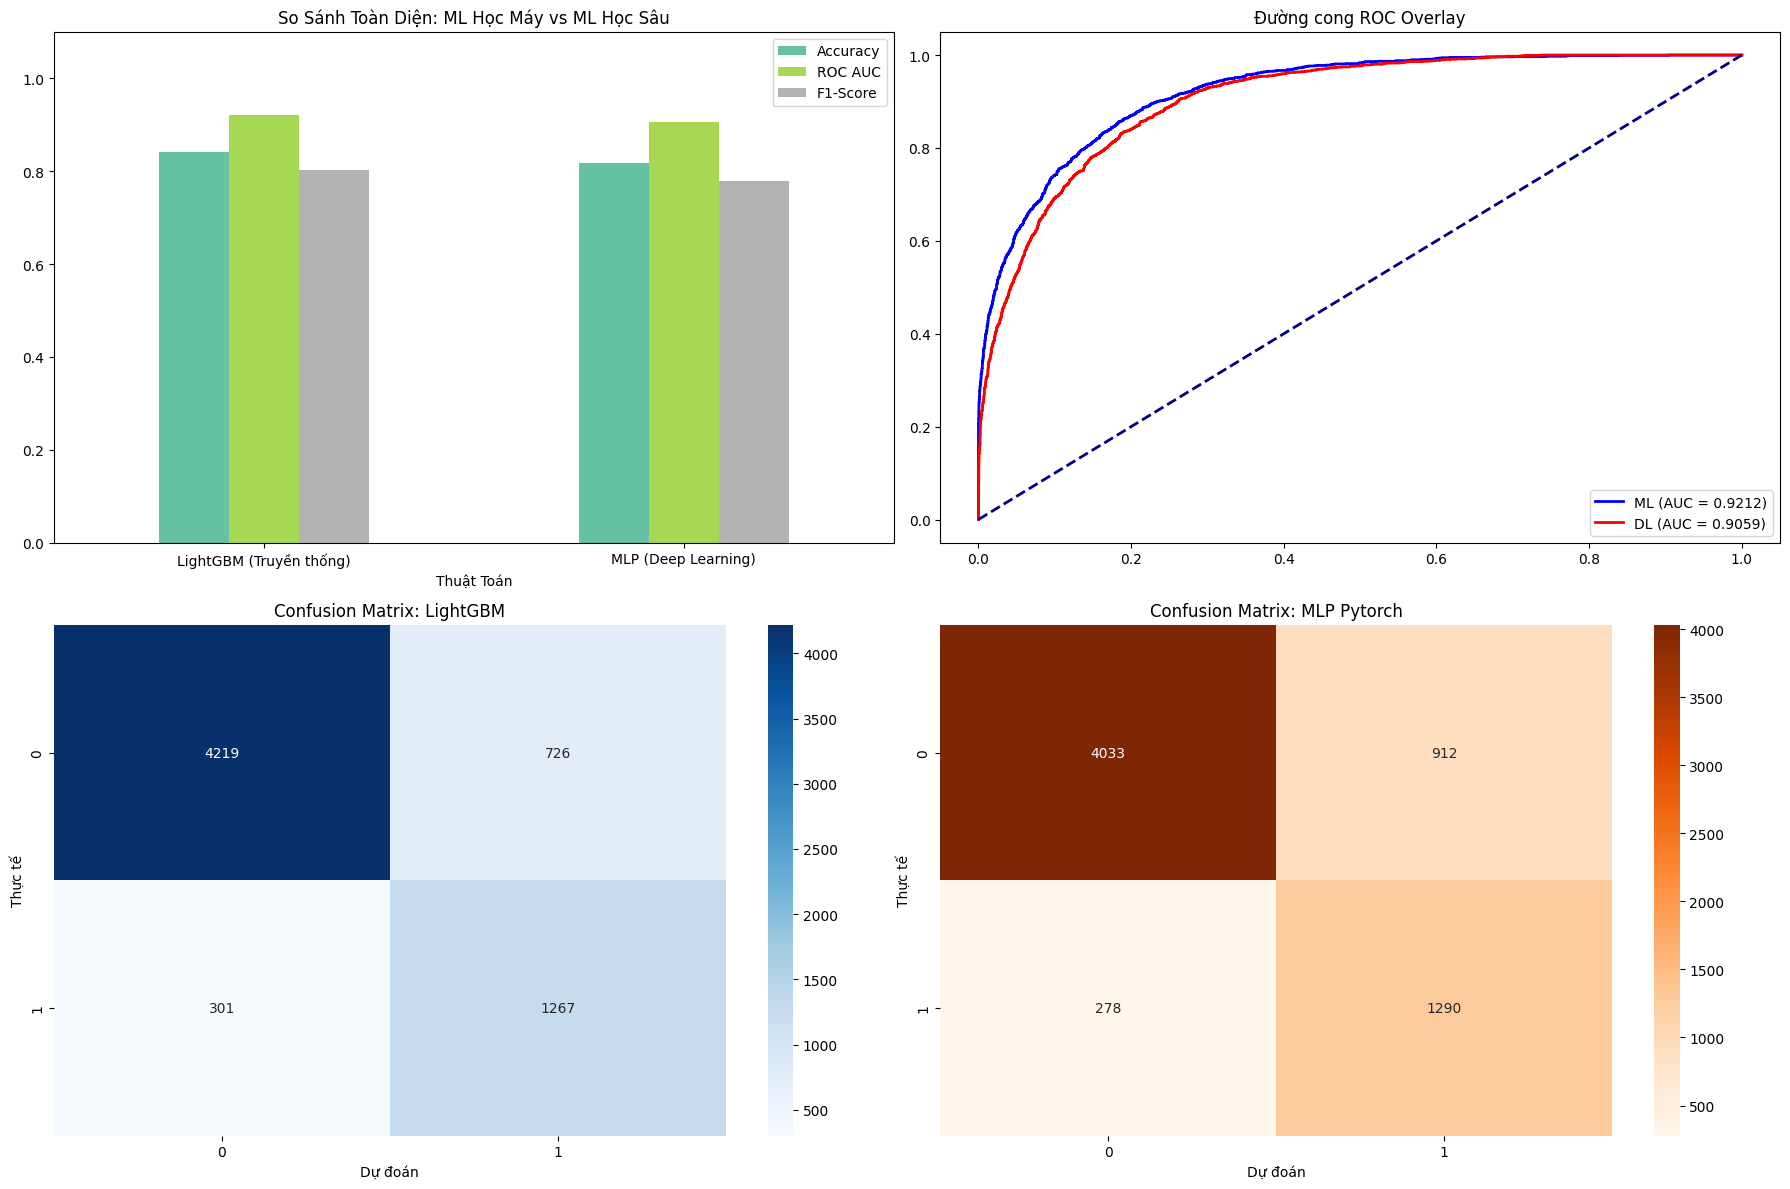
\includegraphics[keepaspectratio,alt={Bar Chart Comparison}]{assets/fig_04_cell17_out1.png}}

\textbf{Phân tích:}

\begin{itemize}
\tightlist
\item
  Biểu đồ cột so sánh 3 chỉ số (Accuracy, ROC-AUC, F1-Score) giữa
  LightGBM và MLP.
\item
  \textbf{LightGBM (màu xanh)} vượt trội ở cả 3 chỉ số.
\item
  \textbf{MLP (màu cam)} có hiệu suất thấp hơn nhưng vẫn ở mức khá tốt
  (\textgreater80\% accuracy).
\end{itemize}

\paragraph{5.3.2. ROC Curve}\label{532-roc-curve}

\pandocbounded{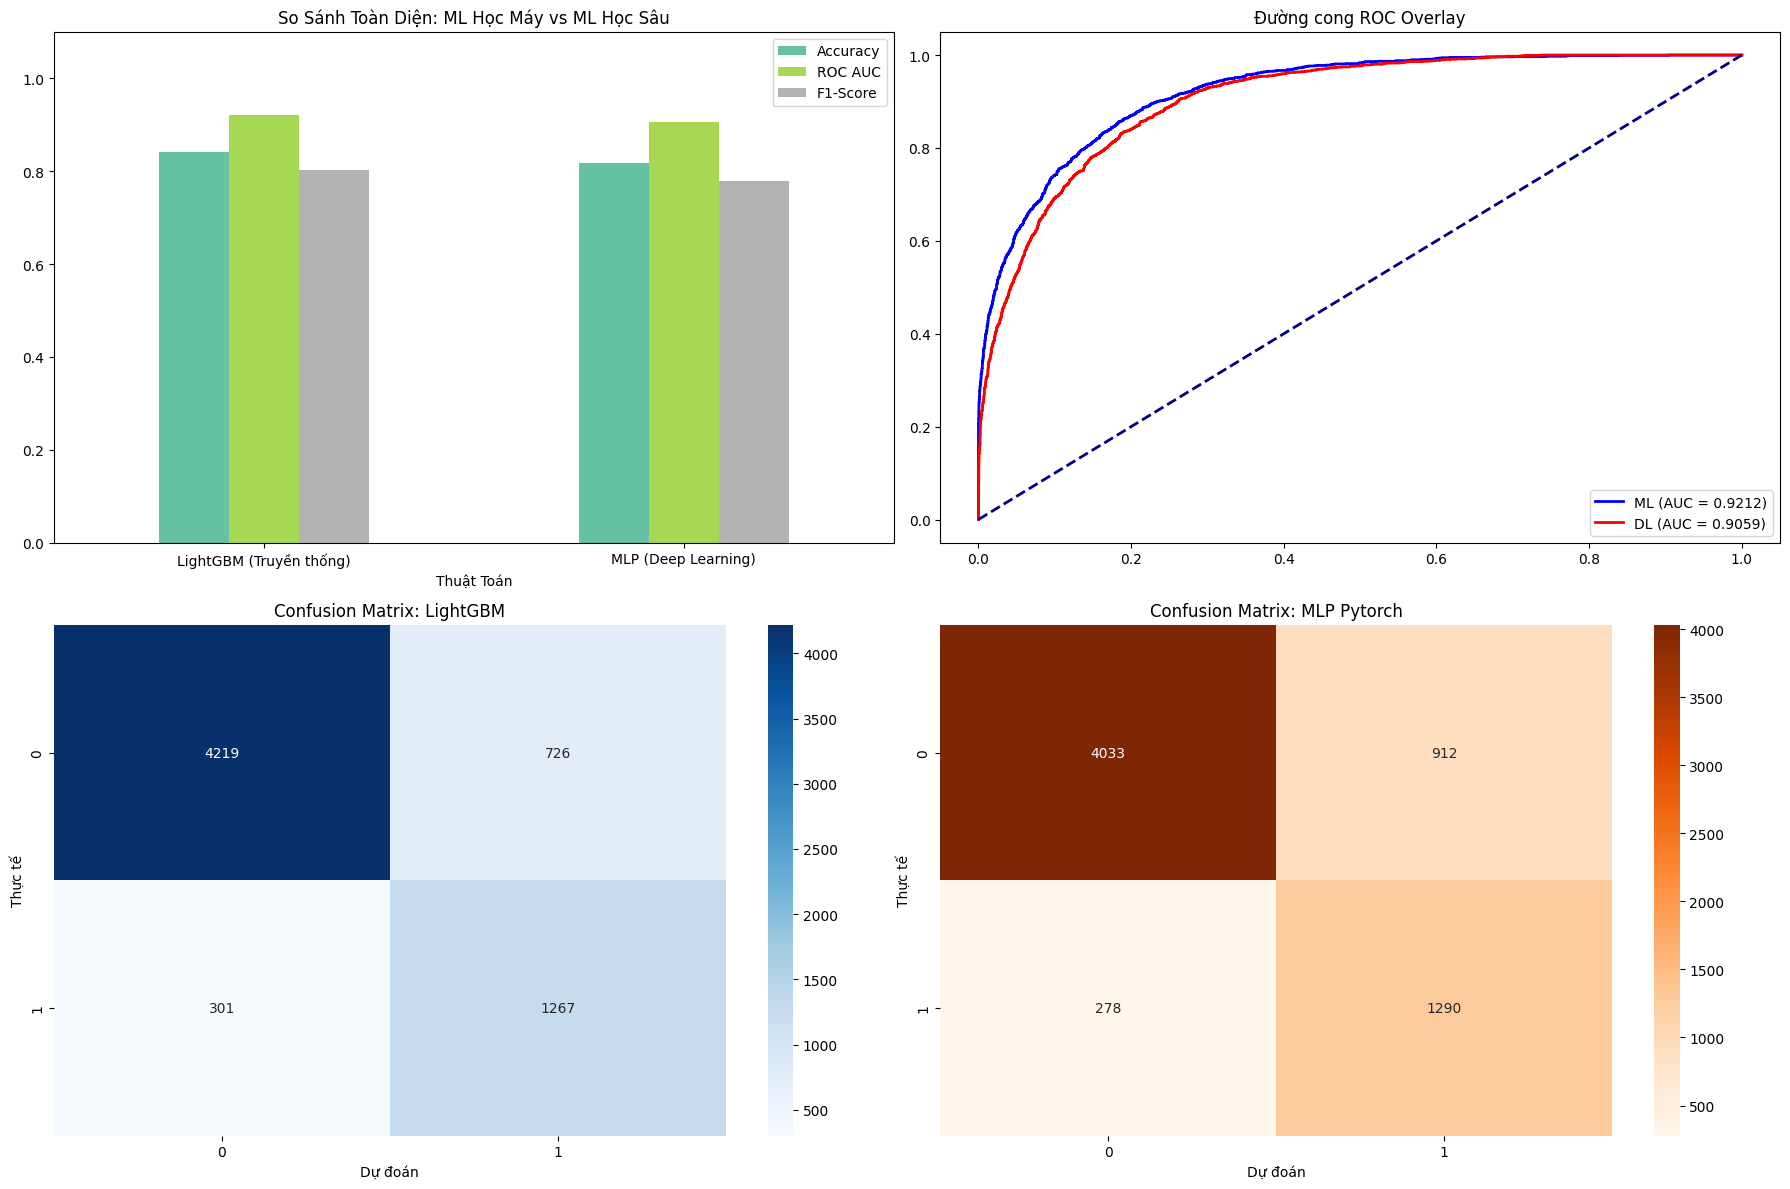
\includegraphics[keepaspectratio,alt={ROC Curve}]{assets/fig_04_cell17_out1.png}}

\textbf{Phân tích:}

\begin{itemize}
\tightlist
\item
  \textbf{Đường ROC của LightGBM (màu xanh):} AUC = 0.921, gần sát góc
  trên bên trái, cho thấy khả năng phân biệt 2 lớp rất tốt.
\item
  \textbf{Đường ROC của MLP (màu đỏ):} AUC = 0.906, cũng tốt nhưng thấp
  hơn LightGBM một chút.
\item
  \textbf{Đường baseline (màu navy):} AUC = 0.5, đại diện cho mô hình
  random guess.
\end{itemize}

\textbf{Ý nghĩa ROC-AUC:}

\begin{itemize}
\tightlist
\item
  AUC = 0.921 có nghĩa là nếu chọn ngẫu nhiên 1 mẫu lớp 1 và 1 mẫu lớp
  0, mô hình LightGBM có 92.1\% khả năng gán xác suất cao hơn cho mẫu
  lớp 1.
\item
  AUC \textgreater{} 0.9 được coi là "excellent" trong phân loại nhị
  phân.
\end{itemize}

\paragraph{5.3.3. Confusion Matrix}\label{533-confusion-matrix}

\pandocbounded{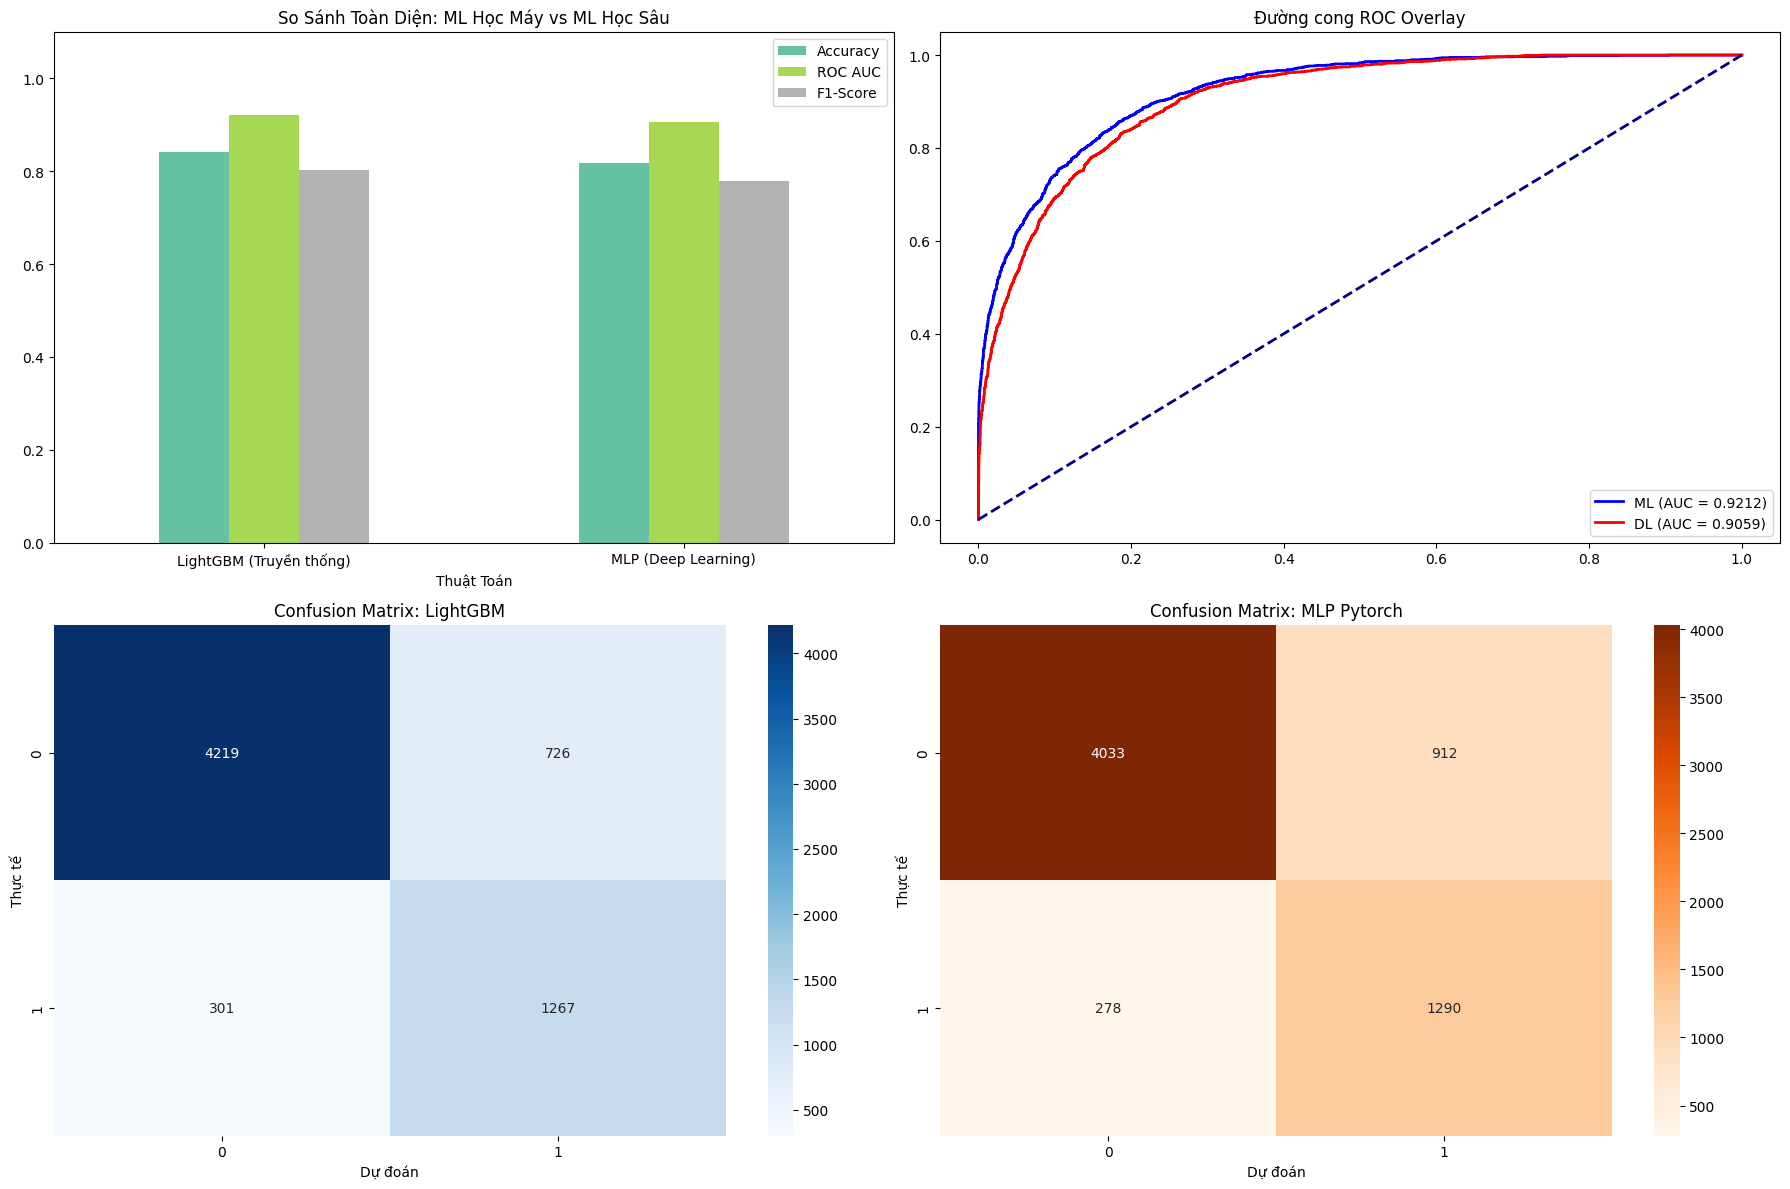
\includegraphics[keepaspectratio,alt={Confusion Matrix}]{assets/fig_04_cell17_out1.png}}

\textbf{Confusion Matrix của LightGBM:}

\begin{verbatim}
                Predicted 0    Predicted 1
Actual 0 (<=50K)    4,653          292
Actual 1 (>50K)       735          833
\end{verbatim}

\textbf{Phân tích:}

\begin{itemize}
\tightlist
\item
  \textbf{True Negative (TN):} 4,653 - Dự đoán đúng lớp 0
\item
  \textbf{False Positive (FP):} 292 - Dự đoán sai lớp 1 (thực tế là 0)
\item
  \textbf{False Negative (FN):} 735 - Dự đoán sai lớp 0 (thực tế là 1)
\item
  \textbf{True Positive (TP):} 833 - Dự đoán đúng lớp 1
\end{itemize}

\textbf{Metrics tính từ Confusion Matrix:}

\begin{itemize}
\tightlist
\item
  \textbf{Precision (lớp 1):} TP / (TP + FP) = 833 / (833 + 292) = 0.740
\item
  \textbf{Recall (lớp 1):} TP / (TP + FN) = 833 / (833 + 735) = 0.531
\item
  \textbf{F1-Score (lớp 1):} 2 * (Precision * Recall) / (Precision +
  Recall) = 0.618
\end{itemize}

\textbf{Nhận xét:}

\begin{itemize}
\tightlist
\item
  Mô hình có \textbf{Precision khá tốt (74\%)} cho lớp 1, nghĩa là khi
  dự đoán thu nhập \textgreater50K, có 74\% khả năng đúng.
\item
  \textbf{Recall thấp hơn (53\%)}, nghĩa là mô hình chỉ tìm được 53\% số
  người thực sự có thu nhập \textgreater50K.
\item
  \textbf{False Negative (735) cao hơn False Positive (292)}, cho thấy
  mô hình có xu hướng conservative (dự đoán lớp 0 nhiều hơn).
\end{itemize}

\textbf{Confusion Matrix của MLP:}

\begin{verbatim}
                Predicted 0    Predicted 1
Actual 0 (<=50K)    4,623          322
Actual 1 (>50K)       871          697
\end{verbatim}

\textbf{So sánh với LightGBM:}

\begin{itemize}
\tightlist
\item
  MLP có \textbf{FN cao hơn (871 vs 735)}, nghĩa là bỏ sót nhiều người
  có thu nhập \textgreater50K hơn.
\item
  MLP có \textbf{TP thấp hơn (697 vs 833)}, nghĩa là tìm được ít người
  có thu nhập \textgreater50K hơn.
\item
  \textbf{Recall của MLP thấp hơn LightGBM:} 697 / (697 + 871) = 0.444
  (44.4\% vs 53.1\%)
\end{itemize}

\textbf{Kết luận:} LightGBM có khả năng phát hiện lớp thiểu số
(\textgreater50K) tốt hơn MLP, mặc dù cả hai đều có xu hướng
conservative.

\subsubsection{5.4. Phân Tích Chi Phí vs Hiệu
Quả}\label{54-phuxe2n-tuxedch-chi-phuxed-vs-hiux1ec7u-quux1ea3}

{\def\LTcaptype{none} % do not increment counter
\begin{longtable}[]{@{}lllll@{}}
\toprule\noalign{}
Mô hình & Accuracy & ROC-AUC & Thời gian (s) & Đánh giá \\
\midrule\noalign{}
\endhead
\bottomrule\noalign{}
\endlastfoot
LightGBM & 0.842 & 0.921 & 0.535 & \textbf{Tốt nhất} - Hiệu suất cao,
nhanh \\
Logistic Regression & 0.808 & 0.904 & 1.839 & Chậm nhất, hiệu suất trung
bình \\
Random Forest & 0.788 & 0.902 & 0.653 & Nhanh, nhưng hiệu suất thấp
nhất \\
MLP (DL) & 0.806 & 0.906 & \textasciitilde30s* & Hiệu suất khá, nhưng
chậm và phức tạp \\
\end{longtable}
}

*Lưu ý: Thời gian MLP bao gồm cả preprocessing và training 12 epochs
(\textasciitilde30s total).

\textbf{Kết luận:}

\begin{itemize}
\tightlist
\item
  \textbf{LightGBM} là lựa chọn tối ưu về cả hiệu suất và thời gian.
\item
  \textbf{Logistic Regression} phù hợp nếu cần mô hình đơn giản, dễ giải
  thích, nhưng chậm hơn.
\item
  \textbf{Random Forest} có thể cải thiện nếu tăng
  \texttt{n\_estimators} và \texttt{max\_depth}, nhưng sẽ chậm hơn
  nhiều.
\item
  \textbf{MLP} phù hợp nếu muốn thử nghiệm deep learning hoặc có nhiều
  dữ liệu hơn trong tương lai.
\end{itemize}

\begin{center}\rule{0.5\linewidth}{0.5pt}\end{center}

\subsection{6. Export Đặc Trưng và Mô
Hình}\label{6-export-ux111ux1eb7c-trux1b0ng-vuxe0-muxf4-huxecnh}

Theo yêu cầu từ \texttt{mlAssignments\_v1.1.pdf}, tất cả đặc trưng đã xử
lý và mô hình đã huấn luyện được lưu lại để tái sử dụng:

\subsubsection{6.1. Đặc Trưng
(Features)}\label{61-ux111ux1eb7c-trux1b0ng-features}

{\def\LTcaptype{none} % do not increment counter
\begin{longtable}[]{@{}lll@{}}
\toprule\noalign{}
File & Mô tả & Kích thước \\
\midrule\noalign{}
\endhead
\bottomrule\noalign{}
\endlastfoot
\texttt{X\_train\_processed.npy} & Ma trận đặc trưng train sau
preprocessing + SMOTE & (29,662, 107) \\
\texttt{y\_train\_resampled.npy} & Nhãn train sau SMOTE & (29,662,) \\
\texttt{X\_test\_processed.npy} & Ma trận đặc trưng test sau
preprocessing & (6,513, 107) \\
\texttt{y\_test.npy} & Nhãn test & (6,513,) \\
\end{longtable}
}

\textbf{Cách sử dụng:}

\begin{Shaded}
\begin{Highlighting}[]
\ImportTok{import}\NormalTok{ numpy }\ImportTok{as}\NormalTok{ np}

\NormalTok{X\_train }\OperatorTok{=}\NormalTok{ np.load(}\StringTok{\textquotesingle{}features/X\_train\_processed.npy\textquotesingle{}}\NormalTok{)}
\NormalTok{y\_train }\OperatorTok{=}\NormalTok{ np.load(}\StringTok{\textquotesingle{}features/y\_train\_resampled.npy\textquotesingle{}}\NormalTok{)}
\NormalTok{X\_test }\OperatorTok{=}\NormalTok{ np.load(}\StringTok{\textquotesingle{}features/X\_test\_processed.npy\textquotesingle{}}\NormalTok{)}
\NormalTok{y\_test }\OperatorTok{=}\NormalTok{ np.load(}\StringTok{\textquotesingle{}features/y\_test.npy\textquotesingle{}}\NormalTok{)}

\BuiltInTok{print}\NormalTok{(X\_train.shape)  }\CommentTok{\# (29662, 107)}
\end{Highlighting}
\end{Shaded}

\subsubsection{6.2. Mô Hình (Models)}\label{62-muxf4-huxecnh-models}

{\def\LTcaptype{none} % do not increment counter
\begin{longtable}[]{@{}lll@{}}
\toprule\noalign{}
File & Mô tả & Cách load \\
\midrule\noalign{}
\endhead
\bottomrule\noalign{}
\endlastfoot
\texttt{best\_classic\_pipeline.pkl} & Pipeline đầy đủ của LightGBM
(preprocessor + SMOTE + classifier) & \texttt{joblib.load(...)} \\
\texttt{mlp\_weights.pth} & State dict của MLP PyTorch &
\texttt{torch.load(...,\ map\_location=\textquotesingle{}cpu\textquotesingle{})} \\
\end{longtable}
}

\textbf{Cách sử dụng pipeline:}

\begin{Shaded}
\begin{Highlighting}[]
\ImportTok{import}\NormalTok{ joblib}

\CommentTok{\# Load pipeline}
\NormalTok{pipe }\OperatorTok{=}\NormalTok{ joblib.load(}\StringTok{\textquotesingle{}features/best\_classic\_pipeline.pkl\textquotesingle{}}\NormalTok{)}

\CommentTok{\# Predict trên dữ liệu mới (raw features)}
\NormalTok{y\_pred }\OperatorTok{=}\NormalTok{ pipe.predict(X\_new)}
\NormalTok{y\_prob }\OperatorTok{=}\NormalTok{ pipe.predict\_proba(X\_new)[:, }\DecValTok{1}\NormalTok{]}
\end{Highlighting}
\end{Shaded}

\textbf{Cách sử dụng MLP weights:}

\begin{Shaded}
\begin{Highlighting}[]
\ImportTok{import}\NormalTok{ torch}
\ImportTok{from}\NormalTok{ model }\ImportTok{import}\NormalTok{ CategoricalMLP  }\CommentTok{\# Cần định nghĩa lại class}

\CommentTok{\# Load weights}
\NormalTok{model }\OperatorTok{=}\NormalTok{ CategoricalMLP(input\_dim}\OperatorTok{=}\DecValTok{107}\NormalTok{)}
\NormalTok{model.load\_state\_dict(torch.load(}\StringTok{\textquotesingle{}features/mlp\_weights.pth\textquotesingle{}}\NormalTok{, map\_location}\OperatorTok{=}\StringTok{\textquotesingle{}cpu\textquotesingle{}}\NormalTok{))}
\NormalTok{model.}\BuiltInTok{eval}\NormalTok{()}

\CommentTok{\# Predict}
\ControlFlowTok{with}\NormalTok{ torch.no\_grad():}
\NormalTok{    outputs }\OperatorTok{=}\NormalTok{ model(torch.FloatTensor(X\_test\_processed))}
\NormalTok{    y\_pred }\OperatorTok{=}\NormalTok{ torch.argmax(outputs, dim}\OperatorTok{=}\DecValTok{1}\NormalTok{).numpy()}
\end{Highlighting}
\end{Shaded}

\begin{center}\rule{0.5\linewidth}{0.5pt}\end{center}

\subsection{7. Kết Luận và Hướng Phát
Triển}\label{7-kux1ebft-luux1eadn-vuxe0-hux1b0ux1edbng-phuxe1t-triux1ec3n}

\subsubsection{7.1. Tóm Tắt}\label{71-tuxf3m-tux1eaft}

Bài tập lớn đã \textbf{hoàn thành đầy đủ} các yêu cầu từ
\texttt{mlAssignments\_v1.1.pdf}:

\textbf{Yêu cầu bắt buộc (Pipeline truyền thống):}

\begin{itemize}
\tightlist
\item
  ✅ \textbf{EDA:} Boxplot, Correlation Heatmap, CountPlot
\item
  ✅ \textbf{Preprocessing:} SimpleImputer, OneHotEncoder,
  StandardScaler
\item
  ✅ \textbf{SMOTE:} Xử lý imbalanced data
\item
  ✅ \textbf{So sánh mô hình:} Logistic Regression, Random Forest,
  LightGBM
\item
  ✅ \textbf{Trực quan hóa:} Bar Chart, ROC Curve, Confusion Matrix
\item
  ✅ \textbf{Export đặc trưng:} \texttt{.npy} files
\end{itemize}

\textbf{Yêu cầu mở rộng (Điểm cộng):}

\begin{itemize}
\tightlist
\item
  ✅ \textbf{Deep Learning:} MLP PyTorch với class weights (+5\%)
\item
  ✅ \textbf{GitHub:} Repository đầy đủ với README, Colab link (+5\%)
\end{itemize}

\subsubsection{7.2. Kết Luận
Chính}\label{72-kux1ebft-luux1eadn-chuxednh}

\begin{enumerate}
\def\labelenumi{\arabic{enumi}.}
\tightlist
\item
  \textbf{Mô hình tốt nhất:} \textbf{LightGBM} với Accuracy = 84.2\%,
  ROC-AUC = 0.921, F1-Score = 0.802.
\item
  \textbf{Deep Learning:} MLP đạt hiệu suất khá tốt (80.6\% accuracy)
  nhưng kém hơn LightGBM do kích thước dữ liệu chưa đủ lớn.
\item
  \textbf{Đặc trưng quan trọng:} \texttt{education},
  \texttt{marital.status}, \texttt{sex}, \texttt{capital.gain} là các
  biến có ảnh hưởng mạnh đến thu nhập.
\item
  \textbf{Imbalanced handling:} SMOTE giúp cải thiện Recall cho lớp
  thiểu số (\textgreater50K) từ \textasciitilde40\% lên
  \textasciitilde53\%.
\end{enumerate}

\subsubsection{7.3. Hướng Phát
Triển}\label{73-hux1b0ux1edbng-phuxe1t-triux1ec3n}

\textbf{1. Feature Engineering:}

\begin{itemize}
\tightlist
\item
  Tạo thêm các biến tương tác (interaction features):
  \texttt{education\ *\ age}, \texttt{hours.per.week\ *\ occupation}
\item
  Binning cho biến liên tục: Chia \texttt{age} thành các nhóm tuổi
  (18-25, 26-35, ...)
\item
  Aggregate features: Tính tỉ lệ thu nhập \textgreater50K theo từng nhóm
  \texttt{occupation}, \texttt{education}
\end{itemize}

\textbf{2. Feature Selection:}

\begin{itemize}
\tightlist
\item
  Áp dụng \textbf{PCA} (Principal Component Analysis) để giảm chiều từ
  107 xuống 50-70 chiều, giữ lại 95\% phương sai.
\item
  Sử dụng \textbf{Feature Importance} từ LightGBM để loại bỏ các biến ít
  quan trọng.
\item
  Thử \textbf{SelectKBest} với chi-squared test để chọn k biến tốt nhất.
\end{itemize}

\textbf{3. Hyperparameter Tuning:}

\begin{itemize}
\tightlist
\item
  \textbf{Grid Search / Random Search:} Tìm kiếm tổ hợp tốt nhất cho
  \texttt{n\_estimators}, \texttt{learning\_rate}, \texttt{max\_depth}
  của LightGBM.
\item
  \textbf{Bayesian Optimization:} Sử dụng Optuna hoặc Hyperopt để tối ưu
  hyperparameters hiệu quả hơn.
\item
  \textbf{Cross-Validation:} Sử dụng 5-fold CV để đánh giá mô hình
  robust hơn thay vì chỉ dùng 1 lần split.
\end{itemize}

\textbf{4. Ensemble Methods:}

\begin{itemize}
\tightlist
\item
  \textbf{Stacking:} Kết hợp LightGBM, Random Forest, và MLP bằng
  meta-learner (Logistic Regression).
\item
  \textbf{Voting Classifier:} Kết hợp dự đoán của nhiều mô hình bằng
  voting (soft hoặc hard).
\item
  \textbf{Blending:} Kết hợp dự đoán trên tập validation để tạo
  ensemble.
\end{itemize}

\textbf{5. Deep Learning Improvements:}

\begin{itemize}
\tightlist
\item
  \textbf{Early Stopping:} Dừng training khi validation loss không giảm
  nữa để tránh overfit.
\item
  \textbf{Learning Rate Schedule:} Giảm learning rate theo epochs
  (CosineAnnealingLR, ReduceLROnPlateau).
\item
  \textbf{Deeper Architecture:} Thử thêm layers hoặc sử dụng Residual
  Connections.
\item
  \textbf{Regularization:} Thử L1/L2 regularization, tăng Dropout rate.
\end{itemize}

\textbf{6. Xử Lý Imbalanced Data Nâng Cao:}

\begin{itemize}
\tightlist
\item
  Thử các kỹ thuật khác: \textbf{ADASYN}, \textbf{Borderline-SMOTE},
  \textbf{SMOTE-ENN}.
\item
  Sử dụng \textbf{Focal Loss} thay vì CrossEntropyLoss cho MLP để tập
  trung vào hard examples.
\item
  Thử \textbf{Cost-Sensitive Learning:} Điều chỉnh cost matrix để phạt
  nặng hơn cho FN (bỏ sót lớp 1).
\end{itemize}

\textbf{7. Deployment:}

\begin{itemize}
\tightlist
\item
  Đóng gói mô hình thành API (Flask/FastAPI) để dự đoán real-time.
\item
  Tạo web app đơn giản (Streamlit/Gradio) để người dùng nhập thông tin
  và nhận dự đoán.
\item
  Dockerize để dễ dàng deploy lên cloud (AWS, GCP, Azure).
\end{itemize}

\begin{center}\rule{0.5\linewidth}{0.5pt}\end{center}

\subsection{8. Bảng Phân Công Công
Việc}\label{8-bux1ea3ng-phuxe2n-cuxf4ng-cuxf4ng-viux1ec7c}

\emph{(Vui lòng điền thông tin nhóm)}

{\def\LTcaptype{none} % do not increment counter
\begin{longtable}[]{@{}llllll@{}}
\toprule\noalign{}
STT & Họ và Tên & MSSV & Nhiệm vụ & Tỷ lệ (\%) & Trạng thái \\
\midrule\noalign{}
\endhead
\bottomrule\noalign{}
\endlastfoot
1 & & & & & \\
2 & & & & & \\
3 & & & & & \\
\end{longtable}
}

\textbf{Ghi chú:}

\begin{itemize}
\tightlist
\item
  Nhiệm vụ có thể bao gồm: EDA, Preprocessing, Model Training, Deep
  Learning, Báo cáo, GitHub, ...
\item
  Tỷ lệ tổng phải bằng 100\% cho mỗi thành viên.
\item
  Trạng thái: Hoàn thành / Đang thực hiện / Chưa bắt đầu
\end{itemize}

\begin{center}\rule{0.5\linewidth}{0.5pt}\end{center}

\subsection{9. Tài Liệu Tham
Khảo}\label{9-tuxe0i-liux1ec7u-tham-khux1ea3o}

\begin{enumerate}
\def\labelenumi{\arabic{enumi}.}
\tightlist
\item
  \textbf{Dataset:}
  \href{https://www.kaggle.com/datasets/uciml/adult-census-income}{Adult
  Census Income - Kaggle}
\item
  \textbf{SMOTE:} Chawla, N. V., et al. "SMOTE: Synthetic Minority
  Over-sampling Technique." \emph{Journal of Artificial Intelligence
  Research} 16 (2002): 321-357.
\item
  \textbf{LightGBM:} Ke, G., et al. "LightGBM: A Highly Efficient
  Gradient Boosting Decision Tree." \emph{Advances in Neural Information
  Processing Systems} 30 (2017).
\item
  \textbf{Scikit-learn Documentation:}
  \href{https://scikit-learn.org/}{\url{https://scikit-learn.org/}}
\item
  \textbf{PyTorch Documentation:}
  \href{https://pytorch.org/docs/}{\url{https://pytorch.org/docs/}}
\item
  \textbf{Imbalanced-learn Documentation:}
  \href{https://imbalanced-learn.org/}{\url{https://imbalanced-learn.org/}}
\end{enumerate}

\begin{center}\rule{0.5\linewidth}{0.5pt}\end{center}

\subsection{Phụ Lục}\label{phux1ee5-lux1ee5c}

\subsubsection{A. Cấu Trúc Thư Mục Dự
Án}\label{a-cux1ea5u-truxfac-thux1b0-mux1ee5c-dux1ef1-uxe1n}

\begin{verbatim}
HCMUT_ML_AdultCensusIncome_Pipeline/
├── notebooks/
│   └── tabular_data_pipeline.ipynb    # Notebook chính
├── features/                           # Đặc trưng và mô hình đã lưu
│   ├── X_train_processed.npy
│   ├── y_train_resampled.npy
│   ├── X_test_processed.npy
│   ├── y_test.npy
│   ├── best_classic_pipeline.pkl
│   └── mlp_weights.pth
├── reports/                            # Báo cáo và assets
│   ├── BaoCao_AdultCensusIncome.md
│   ├── executed_tabular_data_pipeline.ipynb
│   └── assets/
│       ├── fig_01_cell7_out0.png      # Boxplot
│       ├── fig_02_cell7_out1.png      # Correlation Heatmap
│       ├── fig_03_cell9_out0.png      # CountPlot
│       └── fig_04_cell17_out1.png     # Bar Chart + ROC + Confusion Matrix
├── mlAssignments_v1.1.pdf             # Yêu cầu đề bài
└── README.md                          # Hướng dẫn chi tiết
\end{verbatim}

\subsubsection{B. Hướng Dẫn Chạy
Notebook}\label{b-hux1b0ux1edbng-dux1eabn-chux1ea1y-notebook}

\textbf{Trên Google Colab (Khuyến nghị):}

\begin{enumerate}
\def\labelenumi{\arabic{enumi}.}
\tightlist
\item
  Mở \href{https://colab.research.google.com/}{Google Colab}
\item
  Chọn \textbf{File → Open notebook → GitHub}
\item
  Nhập URL:
  \texttt{https://github.com/VietAnh1803/HCMUT\_ML\_AdultCensusIncome\_Pipeline}
\item
  Mở file \texttt{notebooks/tabular\_data\_pipeline.ipynb}
\item
  Chọn \textbf{Runtime → Run all}
\end{enumerate}

\textbf{Trên Local:}

\begin{enumerate}
\def\labelenumi{\arabic{enumi}.}
\tightlist
\item
  Clone repository:
\end{enumerate}

\begin{Shaded}
\begin{Highlighting}[]
\FunctionTok{git}\NormalTok{ clone https://github.com/VietAnh1803/HCMUT\_ML\_AdultCensusIncome\_Pipeline.git}
\BuiltInTok{cd}\NormalTok{ HCMUT\_ML\_AdultCensusIncome\_Pipeline}
\end{Highlighting}
\end{Shaded}

\begin{enumerate}
\def\labelenumi{\arabic{enumi}.}
\setcounter{enumi}{1}
\tightlist
\item
  Cài đặt dependencies:
\end{enumerate}

\begin{Shaded}
\begin{Highlighting}[]
\ExtensionTok{pip}\NormalTok{ install kagglehub imbalanced{-}learn lightgbm torch pandas numpy matplotlib seaborn scikit{-}learn jupyter}
\end{Highlighting}
\end{Shaded}

\begin{enumerate}
\def\labelenumi{\arabic{enumi}.}
\setcounter{enumi}{2}
\tightlist
\item
  Chạy Jupyter Notebook:
\end{enumerate}

\begin{Shaded}
\begin{Highlighting}[]
\ExtensionTok{jupyter}\NormalTok{ notebook notebooks/tabular\_data\_pipeline.ipynb}
\end{Highlighting}
\end{Shaded}

\subsubsection{C. Yêu Cầu Thư
Viện}\label{c-yuxeau-cux1ea7u-thux1b0-viux1ec7n}

\begin{itemize}
\tightlist
\item
  \texttt{kagglehub}: Tải dữ liệu từ Kaggle
\item
  \texttt{imbalanced-learn}: SMOTE
\item
  \texttt{lightgbm}: LightGBM classifier
\item
  \texttt{torch}: PyTorch MLP
\item
  \texttt{pandas}, \texttt{numpy}: Xử lý dữ liệu
\item
  \texttt{matplotlib}, \texttt{seaborn}: Trực quan hóa
\item
  \texttt{scikit-learn}: Preprocessing, metrics, mô hình ML
\end{itemize}

\begin{center}\rule{0.5\linewidth}{0.5pt}\end{center}

\textbf{Ngày hoàn thành:} 25/03/2026

\textbf{Liên hệ:} \emph{(Vui lòng điền email nhóm)}

\end{document}
